\documentclass{tstextbook}
\usepackage[]{graphicx}
\usepackage[]{color}

\makeatletter

\usepackage{alltt}

\usepackage{amstext}
\usepackage{amsthm}
\usepackage{amssymb}
\usepackage{blkarray}
\usepackage{mathtools}

\usepackage[hidelinks]{hyperref} % hidelinks removes red boxes around links in some pdf viewers

\renewcommand*{\proofname}{Beweis}

% this is used to draw inside of matrices.

\usepackage{blkarray}
\usetikzlibrary{positioning}
\usepackage{tikz}
\usetikzlibrary{fit, tikzmark}

\newcommand\tm[2][]{\tikz[overlay,remember picture,baseline=(#1.base),inner sep=0pt]\node(#1){$#2$};}


\setlength{\parindent}{0pt}

% new Math operatornames
\DeclareMathOperator{\Cov}{Cov}
\DeclareMathOperator{\VC}{VC} % Varianz-Kovarianz
\DeclareMathOperator{\Var}{Var}
\DeclareMathOperator{\rang}{rang}
\DeclareMathOperator{\F}{F} % Verteilung
\DeclareMathOperator{\Bin}{Bin} % Binomial-Verteilung
\DeclareMathOperator{\argmax}{argmax}

% new Commands

\newcommand{\E}{\mathbb E}
\newcommand{\N}{\mathbb N}
\newcommand{\R}{\mathbb R}
\newcommand{\Prob}{\mathbb P}

\newcommand\bigzero{\makebox(0,0){\text{\huge0}}} % makes huge 0

\begin{document}


\tsbook{WORK IN PROGRESS: Studierendenmitschrift zur Vorlesung: Einführung in die Inferenzstatistik}
       {Jim Feller}
       {Cover Designer}
       {2017}
       {xxxxx}{xxx--xx--xxxx--xx--x}{0.0}
       {Publisher}
       {City}

%---------------------------------------------------------------------------
% Chapters
%---------------------------------------------------------------------------

%---------------------------------------------------------------------------

\chapter{Zufallsvektoren und Zufallsmatrizen}

\begin{book}
	Siehe zu diesem Kapitel S. 564-574. in \textit{Rice, J. A. (2007). Mathematical statistics and data analysis. Belmont, CA: Thomson/Brooks/Cole.} 
\end{book}




\begin{remark}
	Wissen: Für $ X_1, \ldots ,X_n $ i.i.d. $ N(\mu,\sigma^{2}), \; \mu\in\mathbb{R}, \; \sigma^2 > 0 $, ist 
	\[ \bar{X}_n = \frac{1}{n} \sum_{i=1}^{n} X_i \sim N\left(\mu, \frac{\sigma^2}{n} \right),
	\] 
	\[ \hat{\sigma}_n^2 = \frac{1}{n-1} \sum_{i=1}^{n} ( X_i - \bar{X}_n)^2 \sim \frac{\sigma^2}{n-1} \chi_{n-1}^2 
	\]  
	und weiters sind $ \bar{X}_n $  und $ \hat{\sigma}^2_n $ unabhängig. Damit ist insbesondere 
	\[ \frac{\sqrt{n}}{\hat{\sigma}_n}(\bar{X}_n-\mu) \sim t_{n-1}.
	\]
	
\end{remark}
 
 
 


\section{Erwartungswerte und Varianz/Kovarianz-Matrizen}


\begin{definition}[Erwartungswert]
	\index{Erwartungswert}
	Für zufällige Vektoren bzw. Matrizen wird der Erwartungswert komponentenweise definiert. Also: \\
	(i) Ist $ X= \left(X_1, \ldots ,X_n\right)^\prime $  ein Zufallsvektor, dann ist 
\[ \mathbb{E}(X) = \begin{pmatrix} \mathbb{E}(X_1)\\
		\mathbb{E}(X_2)\\
		\vdots\\
		\mathbb{E}(X_n)\\
	\end{pmatrix}.
\]
	(ii) Ist $ M=(M_{ij})_{i=1,\, j=1}^{n \;\; m} $ eine zufällige Matrix, dann ist 
	
\[ 
\mathbb{E}(M)= \mathbb{E} \left((M_{ij})\right)_{i=1,\, j=1}^{n \;\; m}	
\]
\end{definition}

\begin{remark}
	Bemerkung: (i) ist ein Spezialfall von (ii), da man den $n$-Vektor
$X$ auch als $n\times1$ Matrix betrachten kann.
\end{remark}

Für Zufallsvariable $Z$ ist der Erwartungswert linear für $a,b\in\mathbb{R}$,
\[
\mathbb{E}(aZ+b)=a\mathbb{E}(Z)+b.
\]

\begin{theorem}[Linearität des Erwartungswertes]
	\label{th:linearitäterwartungswert}
	\index{Erwartungswert!Linearität}	
(i) Sei $X=(X_{1},\ldots,X_{n})^{\prime}$ ein Zufallsvektor, $A$
eine $m\times n$-Matrix und $b$ ein $m$-dimensionaler Vektor, dann
ist 
\[
\mathbb{E}(AX+b)=A\mathbb{E}(X)+b.
\]

(ii) Sei $M$ eine zufällige $(n\times m)$ Matrix,
$A$ eine $k\times n$ Matrix und $B$ eine $k\times m$ Matrix, dann
ist 
\[
\mathbb{E}(AM+B)=A\mathbb{E}(M)+B.
\]

Ist $C$ eine $m\times k$ Matrix und $D$ eine $n\times k$ Matrix,
dann ist 
\[
\mathbb{E}(MC+D)=\mathbb{E}(M)C+D.
\]

\end{theorem}

\begin{proof}
	

Es genügt, (ii) zu zeigen, da (i) ein Spezialfall von (ii) ist. 

Zeige: $\mathbb{E}(AM+B)=A\mathbb{E}(M)+B.$

Vergleiche Eintrag in Zeile $i$ und Spalte $j$ links und rechts.
\begin{align*}
	\left(\mathbb{E}(AM+B)\right)_{ij} & =\mathbb{E}\left((AM+B)_{ij}\right)\\
	& =\mathbb{E}\left((AM)_{ij}+B{}_{ij}\right)\\
	& =\mathbb{E}\left(\sum_{l=1}^{n}A_{il}M{}_{lj}+B{}_{ij}\right)\\
	& =\sum_{l=1}^{n}A_{il}\mathbb{E}\left(M_{lj}\right)+B_{ij}\\
	& =\left(A\mathbb{E}(M)\right)_{ij}+B_{ij}\\
	& =\left(A\mathbb{E}(M)+B\right)_{ij}.
\end{align*}

Zeige: $\mathbb{E}(MC+D)=\mathbb{E}(M)C+D$.
\begin{align*}
	\left(\mathbb{E}(MC+D)\right)_{ij} & =\mathbb{E}\left((MC+D)_{ij}\right)\\
	& =\mathbb{E}\left((MC)_{ij}+D{}_{ij}\right)\\
	& =\mathbb{E}\left(\sum_{l=1}^{m}M_{il}C{}_{lj}+D{}_{ij}\right)\\
	& =\sum_{l=1}^{m}\mathbb{E}\left(M_{il}\right)C_{lj}+D_{ij}\\
	& =\left(\mathbb{E}(M)C\right)_{ij}+D_{ij}\\
	& =\left(\mathbb{E}(M)C+D\right)_{ij}.
\end{align*}

\end{proof}


\begin{example}
	
$X_{1},\ldots,X_{n}$ i.i.d. mit $\mathbb{E}\left(X_{1}\right)=\mu.$

Betrachte $X=\begin{pmatrix}X_{1}\\
	\vdots\\
	X_{n}
\end{pmatrix}.$

\[
\mathbb{E}(X)=\begin{pmatrix}\mathbb{E}(X_{1})\\
	\vdots\\
	\mathbb{E}(X_{n})
\end{pmatrix}= \begin{pmatrix}
	\mu \\ \vdots \\ \mu
\end{pmatrix} = \mu\iota
\]
für $\iota=\begin{pmatrix}1, & \ldots, & 1\end{pmatrix}^{\prime}\in\mathbb{R}^{n}.$

\[
\mathbb{E}\left(\frac{1}{n}\iota^{\prime}X\right)=\frac{1}{n}\iota^{\prime}\mathbb{E}(X)=\frac{1}{n}\iota^{\prime}\mu\iota=\frac{\mu}{n}\underset{=n}{\underbrace{\iota^{\prime}\iota}}=\mu.
\]

\end{example}

\begin{remark}
$  
X =\iota\tikzmarknode{X}{\bar{X}}+(\tikzmarknode{x}{X}-\iota\bar{X)}$
\begin{tikzpicture}[overlay, remember picture,shorten <=1mm,
	nodes={inner sep=1pt, align=center, font=\footnotesize}]
	\draw[<-] (X.south) -- ++ (0.3,-.5) node[below] {orthogonal!};
	\draw[<-] (x.south) -- ++ (-0.3,-.5) node[below]{};
\end{tikzpicture}
\vspace{6ex}
\end{remark}

\begin{example}

\[
\begin{aligned}
\mathbb{E}(\underset{(n\times1)}{\underbrace{\iota\bar{X}}}) & =\mathbb{E}\left(\iota\frac{1}{n}\iota^{\prime}X\right)\\
 & =\frac{1}{n}\iota\iota^{\prime}\mathbb{E}(X)\\
 & =\frac{1}{n}\iota\iota^{\prime}\mu\iota\\
 & =\mu\frac{1}{n}\iota\iota^{\prime}\iota\\
 & =\mu\iota.
\end{aligned}
\]

\end{example}

\begin{example}
	\label{example1.3}

\begin{align*}
\mathbb{E}(X-\iota\bar{X}) & =\mathbb{E}\left(X-\iota\frac{1}{n}\iota^{\prime}X\right)\\
 & =\mathbb{E}\left(\left(I_{n}-\iota\frac{1}{n}\iota^{\prime}\right)X\right)\\
 & =\left(I_{n}-\frac{1}{n}\iota\iota^{\prime}\right)\mathbb{E}(X)\\
 & =\left(I_{n}-\frac{1}{n}\iota\iota^{\prime}\right)\mu\iota\\
 & =\mu\left(\iota-\frac{1}{n}\iota\iota^{\prime}\iota\right)\\
 & =\mu(\iota-\iota)\\
 & =0.
\end{align*}

\end{example}

\begin{definition}[Varianz/Kovarianz-Matrix]
	\label{varianzkovarianzmatrix}
	\index{Varianz/Kovarianz-Matrix}

Ist $X_{(n\times1)}$ ein Zufallsvektor, dann ist die so genannte
Varianz/Kovarianz-Matrix von X die $n\times n$ Matrix
\[
\VC(X)=\left(\VC(X)_{ij}\right)_{i=1\qquad j=1}^{n\qquad\;\;\; n},
\]
wobei 
\[
\VC(X)=\begin{cases}
\Var(X_{i}) & :i=j\\
\Cov(X_{i},X_{j}) & :i\ne j
\end{cases}
\]
mit $1\le i,j\le n.$ 



\[
\VC(X) = 
\begin{blockarray}{(ccccc)}
		\tm[g]{} & \tm[d]{} &  & & \tm[e]{} \\
		\tm[a]{} &  &  & \tm[k]{} &  \\
		&  &  &  &  \\
		& \tm[l]{} & & \tm[u]{} & \tm[f]{}\\
		\tm[b]{} &  &  & \tm[c]{} & \tm[h]{} \\
\end{blockarray}
\]
\begin{tikzpicture}[overlay, remember picture,]
	\node(x)[fit=(a) (b),inner sep=0pt]{};
	\node(y)[fit=(b) (c),inner sep=0pt]{};
	\filldraw[opacity= .5,orange](x.north west)--(x.south west)--(y.south east)--(y.north east)--(x.north east)--cycle;
	
	\node(z)[fit=(d) (e),inner sep=0pt]{};
	\node(i)[fit=(e) (f),inner sep=0pt]{};
	\filldraw[opacity= .5,orange](z.north west)--(z.south west)--(i.south east)--(i.north east)--(z.north east)--cycle;
	
	\node(h)[fit=(g) (h),inner sep=0pt]{};
	\filldraw[opacity=1, gray, ultra thick](h.north west)--(h.south east)--cycle;
	
	\node      (Kovarianzen)       [right=of z] {Kovarianzen};
	\draw[->] (Kovarianzen.west) -- (l);
	\draw[->] (Kovarianzen.west) -- (k);
	
	\node      (Varianzen)       [right=of h] {Varianzen};
	\draw[->] (Varianzen.west) -- (u);
	
\end{tikzpicture}

\end{definition}

\begin{remark}
	Bemerkung: Weil $ \Cov\left(X_i, X_j) \right)= \Cov\left(X_j,X_i \right) $ ist, ist $ \VC(X) $ immer symmetrisch:  \[ (VC(X))^\prime = VC(X) \]
\end{remark}

\begin{remark}
	Bemerkung: Ist $X$ ein $1$-dimensionaler Vektor, dann ist $VC(X)$ die $1\times1$ Matrix $\Var(X).$
\end{remark}

\begin{theorem}
    \[ VC(X)=\mathbb{E}\left((X-\mathbb{E}(X))(X-\mathbb{E}(X))^\prime \right).\]
\end{theorem}

\begin{proof}
    Sei $i,j\in\lbrace1,\ldots,n\rbrace.$

\begin{equation*}
\begin{split}
\left(\mathbb{E}(X-\mathbb{E}(X))(X-\mathbb{E}(X))^\prime\right)_{ij} & = \left(\mathbb{E}(X-\mathbb{E}(X))_i(X-\mathbb{E}(X))_j\right) \\
 & = \left(\mathbb{E}(X_i-\mathbb{E}(X_i))(X_j-\mathbb{E}(X_j))\right) \\
 &= \Cov(X_i,X_j) \\
 &= (VC(X))_{ij}. 
\end{split}
\end{equation*}
Beachte: Für $i=j$ ist $\Cov(X_i,X_j)=\Var(X_i). $
    
\end{proof}

\begin{theorem}
    Ist $X$ ein $n$-dimensionaler Zufallsvektor, $A$ eine $m\times n$ Matrix und $b\in\mathbb{R}^m,$ dann ist $VC(AX+b)=AVC(X)A^\prime$
\end{theorem}
   
        
\begin{proof}
\begin{align*}
    	VC(AX+b) & = \mathbb{E}((AX+b-\mathbb{E}(AX+b))(AX+b-\mathbb{E}(AX+b))^\prime)) \\
    	& = \mathbb{E}((AX+b-(A\mathbb{E}(X)+b)(AX+b-(A\mathbb{E}(X)+b)^\prime)) \\
    	& = \mathbb{E}((AX-A\mathbb{E}(X))(AX-(A\mathbb{E}(X))^\prime)) \\
    	& = \mathbb{E}(A(X-\mathbb{E}(X))(X-(\mathbb{E}(X))^\prime)A^\prime) \\
    	& = A\mathbb{E}((X-\mathbb{E}(X))(X-(\mathbb{E}(X))^\prime)A^\prime) \\
    	& = A\mathbb{E}((X-\mathbb{E}(X))(X-(\mathbb{E}(X))^\prime)A^\prime \\
    	& = A\VC(X)A^\prime.
\end{align*} 
\end{proof}

\begin{example}
	\label{example.vc}
	
	$ X_1,\ldots,X_n $ i.i.d., $ \mathbb{E}{(X_1)}= \mu $, $ \Var(X_1) = \sigma^2 $.
	$ X = \begin{pmatrix}
		X_1 \\ \vdots \\ X_n
	\end{pmatrix} $ 

\[	\mathbb{E}(X) = \begin{pmatrix}
		\mu \\ \vdots \\ \mu
	\end{pmatrix} = \mu\iota. 
\]

\[ \VC(X) = \begin{pmatrix}
		
			\sigma^2 										\\
			& \ddots  		& 			& \text{\huge0}		\\
			& 				& \ddots               			\\
			& \text{\huge0} & 			& \ddots           	\\
			& 				& 			& 		& \sigma^2
		
	\end{pmatrix} = \sigma^2 I_n
\]

Betrachte $ \bar{X},\, X-\iota\bar{X} $. \\
$ \begin{pmatrix}
	\bar{X} \\ X-\iota\bar{X}
\end{pmatrix}\ldots $ ein $ (n+1) $-dimensionaler Vektor.


\[
\begin{pmatrix}\mathbb{E}\left(\bar{X}\right)\\
	\mathbb{E}\begin{pmatrix}X-\iota\bar{X}\end{pmatrix}
\end{pmatrix}=\begin{pmatrix}\mu\\
	O
\end{pmatrix}.
\]

Varianzkovarianzmatrix:

\begin{align*}
	VC\left(Z\right) & =\mathbb{E}\left[\begin{pmatrix}\bar{X}-\mu\\
		X-\iota\bar{X}-0
	\end{pmatrix}\begin{pmatrix}\bar{X}-\mu & \left(X-\iota\bar{X}-0\right)\end{pmatrix}^{\prime}\right]\\
	& =\mathbb{E}\left[\begin{pmatrix}\bar{X}-\mu\\
		X-\iota\bar{X}
	\end{pmatrix}\begin{pmatrix}\left(\bar{X}-\mu\right) & \left(X-\iota\bar{X}\right)\end{pmatrix}^{\prime}\right]\\
	& =\mathbb{E}\left[\begin{pmatrix}\left(\bar{X}-\mu\right)\left(\bar{X}-\mu\right) & \left(\bar{X}-\mu\right)\left(X-\iota\bar{X}\right)^{\prime}\\
		\left(X-\iota\bar{X}\right)\left(\bar{X}-\mu\right) & \left(X-\iota\bar{X}\right)\left(X-\iota\bar{X}\right)^{\prime}
	\end{pmatrix}\right]\\
	& =\begin{pmatrix}\mathbb{E}\left(\bar{X}-\mu\right)^{2} & \mathbb{E}\left(\left(\bar{X}-\mu\right)\left(X-\iota\bar{X}\right)^{\prime}\right)\\
		\mathbb{E}\left(X-\iota\bar{X}\right)\left(\bar{X}-\mu\right) & \mathbb{E}\left(\left(X-\iota\bar{X}\right)\left(X-\iota\bar{X}\right)^{\prime}\right)
	\end{pmatrix}\\
	& =\begin{pmatrix}\textcolor{red}{\Var(\bar{X})} & \textcolor{cyan}{\mathbb{E}\left(\left(\bar{X}-\mu\right)\left(X-\iota\bar{X}\right)^{\prime}\right)}\\
		\textcolor{cyan}{\mathbb{E}\left(X-\iota\bar{X}\right)\left(\bar{X}-\mu\right)} & \textcolor{orange}{\mathbb{E}\left(\left(X-\iota\bar{X}\right)\left(X-\iota\bar{X}\right)^{\prime}\right)}
	\end{pmatrix}.
\end{align*}


\[
\textcolor{red}{\Var(\bar{X})}=\frac{\sigma^{2}}{n}.
\]



\[
\textcolor{cyan}{\mathbb{E}\left(\left(\bar{X}-\mu\right)\left(X-\iota\bar{X}\right)^{\prime}\right)}=?
\]

Zwei Zwischenschritte:

\begin{align*}
	\bar{X}-\mu & =\left(\frac{1}{n}\iota^{\prime}X\right)-\left(\frac{1}{n}\iota^{\prime}\mu\iota\right)\\
	& =\left(\frac{1}{n}\iota^{\prime}X\right)-\left(\frac{1}{n}\iota^{\prime}\mathbb{E}(X)\right)\\
	& =\frac{1}{n}\iota^{\prime}\left(X-\mathbb{E}(X)\right),
\end{align*}

und

\begin{align*}
	X-\iota\bar{X} & =X-\iota\frac{1}{n}\iota^{\prime}X\\
	& =\left(I_{n}-\iota\frac{1}{n}\iota^{\prime}\right)X\\
	& =\left(I_{n}-\iota\frac{1}{n}\iota^{\prime}\right)\left(X-\mathbb{E}(X)\right),
\end{align*}

da
\begin{align*}
	\left(I_{n}-\iota\frac{1}{n}\iota^{\prime}\right)\mathbb{E}(X) & =\left(I_{n}-\iota\frac{1}{n}\iota^{\prime}\right)\mu\iota\\
	& =\mu\left(I_{n}\iota-\frac{1}{n}\iota\iota^{\prime}\iota\right)\\
	& =\mu\left(\iota-\frac{n}{n}\iota\right)\\
	& =\mu\left(\iota-\iota\right)\\
	& =O.
\end{align*}

\begin{align*}
	\mathbb{E}\left(\left(\bar{X}-\mu\right)\left(X-\iota\bar{X}\right)^{\prime}\right) & =\mathbb{E}\left(\left(\frac{1}{n}\iota^{\prime}\left(X-\mathbb{E}(X)\right)\right)\left(\left(X-\mathbb{E}(X)\right)^{\prime}\left(I_{n}-\iota\frac{1}{n}\iota^{\prime}\right)\right)\right)\\
	& =\frac{1}{n}\iota^{\prime}\mathbb{E}\left(\left(\left(X-\mathbb{E}(X)\right)\right)\left(\left(X-\mathbb{E}(X)\right)^{\prime}\right)\right)\left(I_{n}-\iota\frac{1}{n}\iota^{\prime}\right)\\
	& =\frac{1}{n}\iota^{\prime}VC(X)\left(I_{n}-\iota\frac{1}{n}\iota^{\prime}\right)\\
	& =\sigma^{2}\frac{1}{n}\iota^{\prime}\left(I_{n}-\iota\frac{1}{n}\iota^{\prime}\right)\\
	& =\sigma^{2}\frac{1}{n}\left(\iota^{\prime}-\iota^{\prime}\iota\frac{1}{n}\iota^{\prime}\right)\\
	& =\sigma^{2}\frac{1}{n}\left(\iota^{\prime}-\iota^{\prime}\right)\\
	& =O.
\end{align*}


\begin{align*}
	\textcolor{orange}{\mathbb{E}\left(\left(X-\iota\bar{X}\right)\left(X-\iota\bar{X}\right)^{\prime}\right)} & =VC(X-\iota\bar{X})\\
	& =VC(X-\iota\frac{1}{n}\iota^{\prime}X)\\
	& =VC\left(\left(I_{n}-\iota\frac{1}{n}\iota^{\prime}\right)X\right)\\
	& =\left(I_{n}-\iota\frac{1}{n}\iota^{\prime}\right)VC(X)\left(I_{n}-\iota\frac{1}{n}\iota^{\prime}\right)^{\prime}\\
	& =\left(I_{n}-\iota\frac{1}{n}\iota^{\prime}\right)\sigma^{2}\left(I_{n}-\iota\frac{1}{n}\iota^{\prime}\right)^{\prime}\\
	& =\sigma^{2}\left(I_{n}-\iota\frac{1}{n}\iota^{\prime}\right)\left(I_{n}-\iota\frac{1}{n}\iota^{\prime}\right)^{\prime}\\
	& =\sigma^{2}\left(I_{n}-\iota\frac{1}{n}\iota^{\prime}-\iota\frac{1}{n}\iota^{\prime}+\iota\frac{1}{n}\iota^{\prime}\iota\frac{1}{n}\iota^{\prime}\right)\\
	& =\sigma^{2}\left(I_{n}-\iota\frac{1}{n}\iota^{\prime}-\iota\frac{1}{n}\iota^{\prime}+\iota\frac{1}{n}\iota^{\prime}\right)\\
	& =\sigma^{2}\left(I_{n}-\iota\frac{1}{n}\iota^{\prime}\right).
\end{align*}

Also:

\[
VC\begin{pmatrix}
	\bar{X} \\ X-\iota\bar{X}
\end{pmatrix}=\begin{pmatrix}\frac{\sigma^{2}}{n} & O^{\prime}\\
	O^{\prime} & \sigma^{2}\left(I_{n}-\iota\frac{1}{n}\iota^{\prime}\right)
\end{pmatrix}.
\]

Man sieht: $ \bar{X} $ und $ X-\iota\bar{X} $ sind komponentenweise unkorreliert.

\end{example}

\begin{remark}
	Bezeichnung:
Für zwei Zufallsvektoren $ X\in\mathbb{R}^n $ und $ Y\in\mathbb{R}^m $ ist die $ n\times m $ Matrix $ \Cov(X,Y) $ definiert als $ \Cov(X,Y)=\mathbb{E}((X-\mathbb{E}(X))(Y-\mathbb{E}(Y))^\prime). $

Weiters ist die $ m\times n $ Matrix $ \Cov(Y,X) $ definiert als $ \Cov(Y,X)=\mathbb{E}((Y-\mathbb{E}(Y))(X-\mathbb{E}(X))^\prime). $

Beachte: $ \Cov(X,Y) = (\Cov(Y,X))^\prime $
\end{remark}

\begin{remark}
	Bemerkung: Zwei Zufallsvektoren $ X,Y $ sind unabhängig, wenn für beliebige Funktionen $ f(x) $ und $ g(y) $ die Beziehung $ \mathbb{E}(f(x)g(y))=\mathbb{E}(f(x))\mathbb{E}(g(y)) $ gilt.
\end{remark}

\begin{theorem}
	Sind $ X,Y $ unabhängige Zufallsvektoren, dann ist $ \Cov(X,Y)=0. $
\end{theorem}

\begin{proof}
	Siehe Übung.
\end{proof}

\begin{theorem}
	
	Ist $ X $ ein Zufallsvektor mit $ \VC(X)=\Sigma $, dann gilt 
	\[\begin{aligned}
	\Sigma^\prime &=\Sigma, & \text{(symetrisch)} \\
	\Sigma & \ge0. & \text{(positiv semidefinit)}
	\end{aligned}
	\] 
	
\end{theorem}

\begin{proof}
	Sei $ X $ ein $n$-dimensionaler Zufallsvektor. 
	\begin{align*}
	\Sigma^\prime &=(VC(X))^\prime \\
	& = (\mathbb{E}((X-\mathbb{E}))(X-\mathbb{E}(X)^\prime))^\prime \\
	& = \mathbb{E}((X-\mathbb{E}(X))(X-\mathbb{E}(X))^\prime)\\
	& = \VC(X)\\
	& = \Sigma.\checkmark
\end{align*}

$ \Sigma\ge0\ldots $ d.h. für jeden Vektor $ \alpha\in\mathbb{R}^n $ ist $ \alpha^\prime\Sigma\alpha\ge0. $
Sei also $ \alpha\in\mathbb{R}^n\setminus\{0\}. $ Betrachte die Zufallsvariable $ \alpha^\prime X: $

\begin{align*}	
	0 \le \Var(\alpha^\prime X) & = \VC(\alpha^\prime X) \\
	&= \alpha^\prime \VC(X)\alpha\\
	&= \alpha^\prime\Sigma\alpha.\checkmark	
\end{align*}	

\end{proof}

\begin{remark}
	Bemerkung: Ist $ \Sigma = \VC(X) > 0 $, dann ist für jeden Vektor $ \alpha \in \R^n, \, \alpha \ne 0 $, die Varianz von $ \alpha^\prime X $ positiv (und umgekehrt): 
	Für $ \alpha \in \R^n\setminus\{0\} $ ist $ \Var(\alpha^\prime X) = \alpha^\prime \Sigma \alpha $.
\end{remark}

\begin{remark}
	Erinnerung: Sei $ A $ eine symmetrische Matrix $ (n\times n) $. \\
	Seien $ \lambda_1, \ldots, \lambda_n $ die Eigenwerte, und seien $ u_1,\ldots, u_n $ die entsprechenden Eigenvektoren. \\
	Setze $ U = (u_1, u_2, \ldots, u_n)_{(n \times n)}$ , \\
	sowie $ \Omega = \begin{pmatrix}
		\lambda_1 & & 0  \\
		& \ddots \\
		0 & & \lambda_n
	\end{pmatrix}_{(n\times n)} $. \\
	Dann gilt: $ A = U \Omega U^\prime $.
	
\end{remark}

Mit R-Beispiel vom 08.03.2021 (oder auch ganz allgemein) sieht man: \\
Sind $ \lambda_i $ die Eigenwerte und $ u_i $ die Eigenvektoren von $ A_{(n \times n)} $, dann gilt 
	\[
	\begin{aligned}
		&A u_i & = & \lambda_i u_i , \quad 1\le i \le n. &&\\
		&& \equiv & A\underbrace{(u_1,\ldots,u_n)}_U & = & (\lambda_1 u_1, \ldots, \lambda_n u_n) \\
		&& \equiv & A U & = & U\Omega\\
		&&\Rightarrow & A \underbrace{UU^\prime}_{I_n} & = & U\Omega U^\prime 
	\end{aligned}
	\] 
	Also: $ A = U \Omega U^\prime $. 
	\[
	Ax = \tikzmarknode{U}{U} \tikzmarknode{O}{\Omega} \tikzmarknode{UP}{U^\prime} x
	\]
	\begin{tikzpicture}[overlay, remember picture,shorten <=1mm,
		nodes={inner sep=1pt, align=center, font=\footnotesize}]
		\draw[<-] (U.south) -- ++ (-2,-.5) node[below] {Rücktransformation};
		\draw[<-] (O.south) -- ++ (0,-1) node[below] {Stauchung/Streckung};
		\draw[<-] (UP.south) -- ++ (2.2,-2) node[below] {Transformation in neues Koordinatensystem};
	\end{tikzpicture}
	\vspace{10ex}
	
	$ A^2 = AA = U \Omega U^\prime U \Omega U^\prime = U \Omega^2 U^\prime $. \\
	$ A^{\frac{1}{2}} \coloneqq U \tikzmarknode{D}{\Omega^{\frac{1}{2}}} U^\prime $.
	\begin{tikzpicture}[overlay, remember picture,shorten <=1mm,
		nodes={inner sep=1pt, align=center, font=\footnotesize}]
		\draw[<-] (D.south) -- ++ (1,-.5) node[below] {diag$ \left( \sqrt{\lambda_1}, \ldots, \sqrt{\lambda_n} \right) $};
	\end{tikzpicture}
	\vspace{8ex}

	$ A^{\frac{1}{2}} A^{\frac{1}{2}} = U \Omega^{\frac{1}{2}} U^\prime U \Omega^{\frac{1}{2}} U^\prime = U \Omega^{\frac{1}{2}} \Omega^{\frac{1}{2}} U^\prime = A$. \\
	
	Ist $ A $ invertierbar, dann sind alle $ \lambda_i \ne 0 $, sodass $ \Omega^{-1} = \text{diag} \left(\frac{1}{\lambda_1}, \ldots, \frac{1}{\lambda_n} \right)  $ wohldefiniert ist.\\
	Dann ist aber $ A^{-1} = U \Omega^{-1} U^\prime $, denn 
	\[
	\begin{aligned}
		A U \Omega^{-1} U & = U \Omega \underbrace{U^\prime U}_{I_n} \Omega^{-1} U^\prime & = U U^\prime & = I_n. \\
		U \Omega^{-1} U^\prime A & = \ldots & & = I_n.
	\end{aligned}
	\]
	
	Weiters ist dann 
	\[
	A^{-\frac{1}{2}} = U \tikzmarknode{D2}{\Omega^{-\frac{1}{2}}} U^\prime
	\] 
	\begin{tikzpicture}[overlay, remember picture,shorten <=1mm,
		nodes={inner sep=1pt, align=center, font=\footnotesize}]
		\draw[<-] (D2.south) -- ++ (1,-.5) node[below] {diag$ \left( \frac{1}{\sqrt{\lambda_1}}, \ldots, \frac{1}{\sqrt{\lambda_n}} \right) $};
	\end{tikzpicture}
	\vspace{8ex}
	
	ebenfalls wohldefiniert und erfüllt die Beziehung 
	\[
	A^{-\frac{1}{2}} A A^{-\frac{1}{2}} = I_n \quad \text{(Details: Übung.)}
	\]
	
	\begin{remark}
		Bemerkung: Ist $ X $ ein $ n $-dimensionaler Zufallsvektor mit Mittelwert $ 0 $ und VC Matrix $ \Sigma > 0 $, dann gilt für den Zufallsvektor $ Y = \Sigma^{-\frac{1}{2}} X $ ($ n $-dim.): 
		\[ \begin{aligned}
		\E(Y) & = 0 \\
		\VC(Y) & = I_n.
		\end{aligned}
		\]
	\end{remark}
	
	\begin{proof}[Nachrechnen]
	
	\[ \E(Y) = \E\left(\Sigma^{-\frac{1}{2}} X\right) = \Sigma^{-\frac{1}{2}} \E(X) = \Sigma^{-\frac{1}{2}} \cdot 0 = 0 \in \R^n. \checked \]
	
	\[ 
	\begin{aligned}
		\VC(Y) & = \VC\left(\Sigma^{-\frac{1}{2}}X\right) \\
		& = \Sigma^{-\frac{1}{2}} \VC(X) \underbrace{\left(\Sigma^{-\frac{1}{2}}\right)^\prime}_{\text{symmetrisch}} \\
		& = \Sigma^{-\frac{1}{2}} \VC(X) \Sigma^{-\frac{1}{2}} \\
		& = \Sigma^{-\frac{1}{2}} \underbrace{\Sigma}_{\Sigma^{\frac{1}{2}}\Sigma^{\frac{1}{2}}} \Sigma^{-\frac{1}{2}} \\
		& = \underbrace{\Sigma^{-\frac{1}{2}} \Sigma^{\frac{1}{2}}}_{I_n} \underbrace{\Sigma^{\frac{1}{2}} \Sigma^{-\frac{1}{2}}}_{I_n} \\
		& = I_n. \checked
	\end{aligned}
	\]		
	\end{proof}

	\begin{remark}
		Bemerkung: Ist $ Y $ ein Zufallsvektor der Dimension $ n $ mit $ \E(Y) = 0 $ und $ \VC(Y) = I_n $. Sei weiters $ \Sigma_{(n \times n)} $, sodass $ \Sigma^\prime = \Sigma $ und $ \Sigma \ge 0 $. \\
		Für $ X = \Sigma^{\frac{1}{2}} Y $ gilt dann: \[ \E(X) = 0 \] und \[ \VC(X) = \Sigma. \]
	\end{remark}
	
	\begin{proof}[Nachrechnen]
		\[
		\E(X) = \E(\Sigma^{\frac{1}{2}} Y) = \Sigma^{\frac{1}{2}} \E(Y) = \Sigma^{\frac{1}{2}} 0 = 0 \in \R^n. \checked
		\]
		\[ \VC(X) = VC(\Sigma^{\frac{1}{2}} Y) = \Sigma^{\frac{1}{2}} \VC(Y) \Sigma^{\frac{1}{2}} = \Sigma^{\frac{1}{2}} I_n \Sigma^{\frac{1}{2}} = \Sigma^{\frac{1}{2}} \Sigma^{\frac{1}{2}} = \Sigma. \checked \]
	\end{proof}
	
\section{Die Multivariate Normalverteilung}


\begin{definition}
	\index{Normalverteilung!Multivariate}
	
	Sei $A$ eine $n\times k$ Matrix und $b$ ein n-dim. Vektor. 
	
	Seien weiters $Z_{1},\ldots,Z_{k}$ iid. $N(0,1)$-verteilte reellwertige Zufallsvariablen. 
	
	Setze $Z=\left(Z_{1},\ldots,Z_{k}\right)^{\prime}$ und $X=A\cdot Z+b$
	ein $n$- dim. Zufallsvektor.
	
	Die Verteilung von $X$ nennt man die (multivariate) Normalverteilung
	mit Mittelwert $b$ und $VC$ Matrix $AA^{\prime}.$
	
	Kurz: 
	\[
	X\sim N(b,AA^{\prime}).
	\]
	
	Nomination:
	
	\[
	\begin{array}{cc}
		\text{univariat} & \text{multivariat}\\
		\sigma^{2} & \Sigma\\
		\mu & \mu\text{ (Vektor)}
	\end{array}
	\]
	\end{definition}

\begin{theorem}[]
  \label{th:}
  \index{}
 Für $ X\sim N\left(\mu,\Sigma\right) $ gilt:
 
 \[
 \mathbb{E}(X)=\mu,
 \]
 
 \[
 VC(X)=\Sigma.
 \]
\end{theorem}
\begin{proof}
Sei $\mu\in\mathbb{R}^{n}$ und $\Sigma_{(n\times n)}.$

Wähle $Z=\left(Z_{1},\ldots,Z_{n}\right)^{\prime},$ sodass $Z_{1},\ldots,Z_{n}$
i.i.d. $N(0,1).$

Weiters sei $\Sigma^{\frac{1}{2}}$ die ``Wurzel`` von $\Sigma.$

Betrachte $\Sigma^{\frac{1}{2}}Z+\mu.$ 

Laut Definition ist 
\[
\Sigma^{\frac{1}{2}}Z+\mu\sim N\left(\mu,\Sigma^{\frac{1}{2}}\Sigma^{\frac{1}{2}^{\prime}}\right)\equiv N\left(\mu,\Sigma\right).
\]

Damit gilt:
\begin{align*}
	\mathbb{E}(X) & =\mathbb{E}\left(\Sigma^{\frac{1}{2}}Z+\mu\right)\\
	& =\Sigma^{\frac{1}{2}}\underset{0\in\mathbb{R}^{n}}{\underbrace{\mathbb{E}(Z)}}+\mu\\
	& =\mu.
\end{align*}

\begin{align*}
	VC(X) & =VC\left(\Sigma^{\frac{1}{2}}Z+\mu\right)\\
	& =\Sigma^{\frac{1}{2}}VC(Z)\left(\Sigma^{\frac{1}{2}}\right)^{\prime}\\
	& =\Sigma^{\frac{1}{2}}I_{n}\Sigma^{\frac{1}{2}}\\
	& =\Sigma^{\frac{1}{2}}\Sigma^{\frac{1}{2}}\\
	& =\Sigma.
\end{align*}

\end{proof}



\begin{theorem}[Reproduktionseigenschaft]
  \label{th:repoduktionseigenschaft}
  \index{Reproduktionseigenschaft}
  
  Ist $X$ ein $n$-dim. Zufallsvektor mit $X\sim N(\mu,\Sigma),$ ist
  A eine $m\times n$ Matrix und $b$ ein $m$-dim. Vektor, dann ist
  \[
  AX+b\sim N\left(A\mu+b,A\Sigma A^{\prime}\right).
  \]
\end{theorem}
  \begin{proof}
  
  Sei $Z=\left(Z_{1},\ldots,Z_{n}\right)^{\prime}\in\mathbb{R}^{n}$
  mit $Z_{1},\ldots,Z_{n}$ iid. $N(0,1).$
  
  Dann gilt:
  \[
  \Sigma^{\frac{1}{2}}Z+\mu\sim N\left(\mu,\Sigma\right).
  \]
  
  Also:
  \[
  \Sigma^{\frac{1}{2}}Z+\mu\sim X.
  \]
  
  \begin{align*}
  	\Rightarrow AX+b & \sim A\left(\Sigma^{\frac{1}{2}}Z+\mu\right)+b\\
  	& =A\Sigma^{\frac{1}{2}}Z+A\mu+b\\
  	& =\left(A\Sigma^{\frac{1}{2}}\right)Z+(A\mu+b).
  \end{align*}
  
  Laut Definition ist die Verteilung von $\left(A\Sigma^{\frac{1}{2}}\right)Z+(A\mu+b)$
  gegeben durch
  \begin{align*}
  	N\left(A\mu+b,\left(A\Sigma^{\frac{1}{2}}\right)\left(A\Sigma^{\frac{1}{2}}\right)^{\prime}\right) & =N\left(A\mu+b,A\Sigma^{\frac{1}{2}}\left(\Sigma^{\frac{1}{2}}\right)^{\prime}A^{\prime}\right)\\
  	& =N\left(A\mu+b,A\Sigma A^{\prime}\right)\\
  	& \equiv N\left(A\mu+b,A\Sigma A^{\prime}\right).
  \end{align*}
  
  Also:
  \begin{align*}
  	AX+b & \sim A\Sigma^{\frac{1}{2}}Z+A\mu+b\\
  	& \sim N\left(A\mu+b,A\Sigma A^{\prime}\right).
  \end{align*}
\end{proof}
  
 

\begin{remark}
 Bemerkung:

Die $N(\mu,\Sigma)$-Verteilung kann degeneriert sein, nämlich genau
dann, wenn $\Sigma$ nicht vollen Rang hat $\left(N(\mu,0)\equiv\mu\text{ ist ein degenerierter Fall}\right)$.
\end{remark}

Siehe die folgenden Beispiele.

\begin{example}[ $Z\sim N(0,1)$, $A=0$, $b\in\mathbb{R}.$]
  
  
  Laut Definition ist \[X=A_{(1\times1)}Z_{(1\times1)}+b_{(1\times1)}\sim N\left(b,AA^{\prime}\right)=N(b,0).\]
  
  \[
  X=AZ+b=0\cdot Z+b=b.
  \]
  
  Also: $N(b,0)\equiv b.$
  

\end{example}

\begin{example}
	
	Seien $X_{1},\ldots,X_{n}$ reellwertige Zufallsvariablen, i.i.d. mit
	$X_{i}\sim N\left(\mu,\sigma^{2}\right),\,\sigma^{2}>0.$
	
	Setze $X=\left(X_{1},\ldots,X_{n}\right)^{\prime}.$ 
	
	Beachte: 
	\[
	\mathbb{E}(X)=\begin{pmatrix}\mu\\
		\vdots\\
		\mu
	\end{pmatrix}=\mu\iota.
	\]
	
	\[
	VC(X)=\begin{pmatrix}\sigma^{2} &  & 0\\
		& \ddots\\
		0 &  & \sigma^{2}
	\end{pmatrix}=\sigma^{2}I_{n}.
	\]
	
	
	Sei $Z=\left(Z_{1},\ldots,Z_{n}\right)$ mit $Z_{i}$ iid. $N(0,1).$
	
	Betrachte
	\begin{align*}
		\sigma Z+\mu\iota & =\sigma I_{n}Z+\mu\iota\\
		& \sim N\left(\mu\iota,\sigma I_{n}\left(\sigma I_{n}\right)^{\prime}\right)\text{ (aus Def.)}\\
		& \equiv N\left(\mu\iota,\sigma^{2}I_{n}\right).
	\end{align*}
	
	Weiters gilt: $(\sigma Z+\mu\iota)_{i}=\sigma Z_{i}+\mu\sim N\left(\mu,\sigma^{2}\right)\sim X_{i}$, und $(\sigma Z+\mu\iota)_{i}$, $1\le i\le n,$ sind unabhängig, und $X_{i}$, $1\le i\le n,$ sind unabhängig.
	
	Damit ist $X\sim\sigma Z+\mu\iota\sim N\left(\mu\iota,\sigma^{2}I_{n}\right).$
	
	Also ist $X\sim N\left(\mu\iota,\sigma^{2}I_{n}\right).$
	
	Zerlege $X$ in $X=\iota\overline{X}+\left(X-\iota\overline{X}\right)$.
	
	Wissen:
	\begin{align*}
		\iota\overline{X} & =\iota\frac{1}{n}\iota^{\prime}X\\
		& \sim N\left(\iota\frac{1}{n}\iota^{\prime}\mu\iota,\left(\iota\frac{1}{n}\iota^{\prime}\right)\sigma^{2}I_{n}\left(\iota\frac{1}{n}\iota^{\prime}\right)^{\prime}\right)\text{ (aufgrund der Reprod. Eigenschaft)}\\
		& =N\left(\mu\iota\frac{1}{n}\iota^{\prime}\iota,\sigma^{2}\iota\frac{1}{n}\iota^{\prime}\iota\frac{1}{n}\iota^{\prime}\right)\\
		& =N\left(\mu\iota,\frac{\sigma^{2}}{n}\iota\iota^{\prime}\right),
	\end{align*}
	eine Normalverteilung die auf eine Gerade $[\iota]$ konzentriert
	ist.
	
	Analog sieht man:
	$X-\bar{X}\iota\ldots$ eine Normalverteilung in $ [\iota]^\perp. $\\
	Wissen: \\
	\[ \mathbb{E}\left( X-\bar{X}\iota\in\mathbb{R}^n\right) \]
	\[ VC\left(X-\bar{X}\iota\right)=\sigma^2\left(I_n-\iota\frac{1}{n}\iota^{\prime}\right). \]
	Nun ist $ X-\bar{X}\iota=X-\iota\frac{1}{n}\iota^{\prime}X=\left(I_n-\iota \frac{1}{n}\iota^{\prime}\right)X $, sodass \[ X-\iota\bar{X}\sim N\left(0,\sigma^2\left(I_n-\iota\frac{1}{n}\iota^{\prime}\right)\right)\ldots\text{ eine Normalverteilung in}[\iota]^{\perp}.\]
	
	\end{example}

\begin{theorem}
	\index{Normalverteilung!Unabhängigkeit}
	
	Betrachte einen $ m+n $-dimensionalen Zufallsvektor $ \begin{pmatrix} X \\ Y\end{pmatrix} $, wobei $ X \in \mathbb{R}^m $ und $ Y \in \mathbb{R}^n $, sodass 
	\[ \begin{pmatrix}	X \\ Y \end{pmatrix} \sim N(\mu, \Sigma). \]
	Ist $ \operatorname{Cov} (X , Y) = 0 $, dann sind $ X $ und $ Y $ unabhängig.
\end{theorem}

\begin{remark}
	
	Erinnerung: Zufallsvektoren X, Y sind unabhängig, wenn für jede reellwertige Funktion $ f(x) $  und für jede reellwertige Funktion $ g(y) $ die Beziehung $ \mathbb{E}\left(f(x)g(y)\right)=\mathbb{E}\left(f(x)\right) \mathbb{E}\left(g(y)\right)$ gilt.
	
	\end{remark}

\begin{proof}
	
	Partitioniere $ \mu = \mathbb{E} \begin{pmatrix} X \\ Y \end{pmatrix} =  \begin{pmatrix} \mu_X \\ \mu_Y \end{pmatrix}$ mit $ m+n $ Zeilen und $ m+n $ Spalten, sodass
	$  \mathbb{E}(X)=\mu_X $,
	$ \mathbb{E}(Y) = \mu_Y $, sowie
	\[ \Sigma_{((m+n)\times (m+n))} = \begin{pmatrix}
			\Sigma_X & \Sigma_{XY} \\ \Sigma_{YX} & \Sigma_Y
		\end{pmatrix} \], sodass 
	$ VC(X)=\Sigma_X $, $VC(Y)=\Sigma_Y $ und $ \operatorname{Cov}(X,Y) = \Sigma_{XY}. $
	
	Laut Voraussetzung ist $ \Sigma_{XY} = 0 \; (m \times n) $  und $ \Sigma_{YX} = 0 \; (n \times m). $
	Seien $ Z_1,\ldots , Z_{(m+n)} $  i.i.d $ N(0,1) $ und $ Z= \begin{pmatrix}
		 Z_1 \\ \vdots \\ Z_{(m+n)}
	\end{pmatrix} .$ \\
	Partitioniere $ Z =  \begin{pmatrix} Z_X \\ Z_Y \end{pmatrix} $  mit $ m+n $ Zeilen.
	\[ \Sigma^{\frac{1}{2}} = \begin{pmatrix}
		\Sigma_X & 0 \\
		0 & \Sigma_Y
	\end{pmatrix}^{\frac{1}{2}} 
	\stackrel{\hexstar}{=}
	 \begin{pmatrix}
	\Sigma_X^{\frac{1}{2}} & 0 \\
	0 & \Sigma_Y^{\frac{1}{2}}
	\end{pmatrix} \]
Nachrechnen von $ \hexstar $:
	\[ \begin{pmatrix}
		\Sigma_X^{\frac{1}{2}} & 0 \\
		0 & \Sigma_Y^{\frac{1}{2}}
	\end{pmatrix}
	\begin{pmatrix}
		\Sigma_X^{\frac{1}{2}} & 0 \\
		0 & \Sigma_Y^{\frac{1}{2}}
	\end{pmatrix}
	=
	\begin{pmatrix}
		\Sigma_X & 0 \\
		0 & \Sigma_Y
	\end{pmatrix}. \checkmark \] \\

Betrachte den Zufallsvektor 
	\begin{align*}
	 \Sigma^{\frac{1}{2}} Z + \mu & \sim N\left(\mu , \Sigma^{\frac{1}{2}} \Sigma^{\frac{1}{2}} \right) \\ 
	& = 
	N\left(\mu , \Sigma \right) \\
	& \sim 
	\begin{pmatrix}
		X \\ Y
	\end{pmatrix}. 
\end{align*}
	Beachte:
	\begin{align*}
		\Sigma^{\frac{1}{2}} Z + \mu & = \begin{pmatrix}
			\Sigma_X^{\frac{1}{2}} & 0 \\
			0 & \Sigma_Y^{\frac{1}{2}}
		\end{pmatrix} \begin{pmatrix} Z_X \\ Z_Y \end{pmatrix} + \begin{pmatrix} \mu_X \\ \mu_Y \end{pmatrix}\\
	& = \begin{pmatrix}
		\Sigma_X^{\frac{1}{2}} Z_X + \mu_X \\
		\Sigma_Y^{\frac{1}{2}} Z_Y + \mu_Y
	\end{pmatrix} \sim \begin{pmatrix}
	X \\ Y \end{pmatrix}.
	\end{align*}

Nun sind $ Z_X, Z_Y $ unabhängig. \\
$ \Rightarrow \Sigma_X^{\frac{1}{2}} Z_X + \mu_X, \Sigma_Y^{\frac{1}{2}} Z_Y + \mu_Y \text{ unabhängig}. $ \\
$ \Rightarrow X,Y \text{ unabhängig}. $ \\
Zu zeigen: $ X, Y $ unabhängig. \\
Sei: $ f(x) $ eine reellwertige Funtion von $ X $ und $ g(y) $ eine reellwertige Funktion von Y.
Zu zeigen: $ \E(f(x)g(y)) = \E(f(x))E(g(y)). $

\begin{align*} \mathbb{E}(f(x)g(y)) & = \mathbb{E}\left( f\left( \Sigma_X^{\frac{1}{2}} Z_X + \mu_X \right)g\left( \Sigma_Y^{\frac{1}{2}} Z_Y + \mu_Y \right) \right) \\
	& = \mathbb{E}\left( f\left( \Sigma_X^{\frac{1}{2}} Z_X + \mu_X \right)\right) \mathbb{E}\left( g\left( \Sigma_Y^{\frac{1}{2}} Z_Y + \mu_Y \right)\right) \\
	& = \mathbb{E}(f(x)) \mathbb{E}(g(y)).
\end{align*}
\end{proof}

\begin{example}
	$ X_1, \ldots, X_n $ i.i.d. $ N(\mu, \sigma^2), \mu \in \R, 0 < \sigma^2 < \infty $.
	Setze $ X = \begin{pmatrix}
		X_1 \\ \vdots \\ X_n
	\end{pmatrix} \sim N(\mu\iota, \sigma^2 I_n) $.

	Wissen:  
	\[
	\begin{aligned}
	\begin{pmatrix}
		\bar{X} \\ X- \iota \bar{X}
	\end{pmatrix} & \ldots \quad \text{eine lineare Funktion von } X \\
	& = \begin{pmatrix}
		\frac{1}{n} \iota^\prime \\ I_n - \iota \frac{1}{n} \iota^\prime
	\end{pmatrix} X \sim \quad \text{Normalverteilung.}
	\end{aligned}
	\] 
	
	Siehe Beispiel \href{example1.3}{\ref{example1.3}} und \href{example.vc}{\ref{example.vc}}.
	
	$ \Rightarrow \bar{X}, X-\iota\bar{X} $ sind unabhängig!\\
	$ \Rightarrow \bar{X}, \hat{\sigma}_n^2 = \frac{1}{n-1} \sum_{i=1}^{n} (X_i-\bar{X})^2 =  ||X-\iota\bar{X}||^2 $ sind unabhängig!
\end{example}

\begin{remark}
	Erinnerung: Für $ Z_1, \ldots, Z_n $ i.i.d. $ N(0,1) $, ist 
	\[
	\sum_{i=1}^{n} Z_i^2 \sim \chi_k^2.
	\]
\end{remark}
\begin{lemma}
	\index{Orthogonalprojektion}
	
	Ist $ P_{(n \times n)} $ die Matrix einer Orthogonalprojektion, dann gilt: $ P^2=P $  und $ P=P^\prime $.
\end{lemma}

\begin{proof}
	Für $ X,Y \in \R^n $ ist 
	\[ \begin{aligned}
		X & = PX + (I_n - P)X \quad \text{(orthogonale Zerlegung).} \\
		Y & = PY + (I_n - P)Y \quad \text{(orthogonale Zerlegung).}
	\end{aligned}	
	\]
	
	\[
	\begin{aligned}
		X^\prime PY & = (X)^\prime PY \\
		& = (PX+(I_n-P)X)^\prime PY \\
		& = (X^\prime P^\prime +X^\prime(I_n-P)^\prime)PY \\
		& = X^\prime P^\prime PY + \underbrace{X^\prime (I_n-p)^\prime PY}_{\substack{=((I_n-P)X)^\prime PY \\ = 0}} \\
		& = X^\prime P^\prime PY.
	\end{aligned}
	\]
	
	\[
	\begin{aligned}
		X^\prime P^\prime Y & = (PX)^\prime Y \\
		& = (PX)^\prime (PY + (I_n - P)Y) \\
		& = (X^\prime P^\prime (PY + (I_n - P)Y)\\
		& = X^\prime P^\prime PY + \underbrace{X^\prime P^\prime (I_n-P)Y}_{\substack{=(PX)^\prime (I_n-P)Y \\ = 0}} \\
		& = X^\prime P^\prime PY.
	\end{aligned}
	\] 
	
	$ \Rightarrow X^\prime PY = X^\prime P^\prime Y. $  \\
	
	Da dies für beliebige $ X, Y \in \R^n  $ gilt, folgt $ P = P^\prime $. \\
	
	Weiters ist $ X^\prime PY = X^\prime P^\prime PY $ \\
	
	$ \Rightarrow P = P^\prime P \tikzmarknode{P}{=} PP = P^2 $.
	\begin{tikzpicture}[overlay, remember picture,shorten <=1mm,
		nodes={inner sep=1pt, align=center, font=\footnotesize}]
		\draw[<-] (P.south) -- ++ (0,-.5) node[below] {$ P^\prime = P $};
	\end{tikzpicture}
	\vspace{4ex}
	
\end{proof}

\begin{remark}
	Es gilt auch die Umkehrung:
		Ist $ P_{(n \times n)} $ mit $ P^2=P $  und $ P=P^\prime $, dann ist $ P $ die Matrix einer Orthogonalprojektion (ohne Beweis).
	\end{remark}



\begin{corollary}
	
	Ist $ P_{(n\times n)} $ die Matrix einer Orthogonalprojektion auf einen $ k $-dimensionalen Teilraum $ (0 \le k \le n) $, dann sind genau $ k $ Eigenwerte von $ P $ gleich 1 und der Rest ist 0.
	
\end{corollary}

\begin{proof}
	Spektralzerlegung $ P = U \Omega U^\prime $ $ (U \, \text{orthogonal}: U^\prime U = U U^\prime = I_n, \quad \Omega = \text{diag}(\lambda_1,\ldots, \lambda_n)) $. 
	$ P^2 = P $, d.h. 
	\[
	\begin{aligned}
		U\Omega U^\prime U \Omega U^\prime & = U\Omega U^\prime \\
		\Leftrightarrow U \Omega^2 U^\prime &= U \Omega U^\prime \\
		\Leftrightarrow U \Omega^2 &= U \Omega \\
		\Leftrightarrow \Omega^2 &= \Omega.
	\end{aligned}
	\]
	D.h. für $ i=1,\ldots, n  $ ist $ \lambda_i^2 = \lambda_i $, also $ \lambda_i = 0 $ oder $ \lambda_i = 1 $. \\
	Weiters ist  
	\[
	\begin{aligned}	
	\rang(P) & = k \\
	& = \rang(U \Omega U^\prime) \\
	& = \rang(\Omega) \\
	& = \# \{i: 1\le i \le n, \lambda_i = 1\}.
	\end{aligned}
	\]  
	Also sind genau $ k $ Eigenwerte gleich $ 1 $ und $ n-k $ Eigenwerte sind $ 0 $.
\end{proof}
	

\begin{theorem}
	
		Ist $ P_{(n\times n)} $ die Matrix einer Orthogonalprojektion auf einen $ k $-dimensionalen Teilraum $ (1 \le k \le n) $, und ist $ Z \sim N\left(0,1 \right) $. Dann gilt \[ Z^\prime PZ\sim \chi_k^2 \]
	
	\end{theorem}

\begin{proof}
	$ Z^\prime PZ = Z^\prime U \Omega U^\prime Z $. \\
	Nun ist  $ U^\prime Z \sim N(\underbrace{U^\prime 0}_{=0}, \underbrace{U^\prime I_n U}_{\substack{= U^\prime U \\ = I_n}}) \equiv N(0, I_n) $. \\
	
	Insbesondere ist $ Z \sim U^\prime Z $. Für $ \Omega = \text{diag}(\underbrace{1, \ldots, 1}_k, \underbrace{0, \ldots, 0}_{n-k}) $ ist damit 
	\[
	\begin{aligned}
		Z^\prime P Z & = Z^\prime U \Omega U^\prime Z \\
		& = (U^\prime Z)^\prime \Omega (U^\prime Z) \\
		& \sim Z^\prime \Omega Z \\
		& = \sum_{i=1}^{k} Z_i^2 \\
		& \sim \chi_k^2.
	\end{aligned}
	\]
\end{proof}

\begin{example}
	
	Seien $ X_1, \ldots, X_n $ i.i.d. $ N(\mu, \sigma^2) $, sodass $ X = \begin{pmatrix}
		X_1 \\ \vdots \\ X_n
	\end{pmatrix} \sim N(\mu^2. \sigma^2 I_n) $. \\
	
	$ X - \iota\bar{X}  = \underbrace{\left(I_n - \iota \frac{1}{n} \iota^\prime\right)}_{\coloneqq P} X \ldots $ Orthogonalprojektion von $ X $ auf $ [\iota]^\perp $, ein $ (n-1) $.dimensionaler Teilraum.
	
	Prüfe Eigenschaften: 
	\[
	\begin{aligned}
		P^2 & = \left(I_n - \iota \frac{1}{n} \iota^\prime\right)\left(I_n - \iota \frac{1}{n} \iota^\prime\right) \\
		& = I_n - \iota \frac{1}{n} \iota^\prime - \iota \frac{1}{n} \iota^\prime + \iota \frac{1}{n} \iota^\prime \iota \frac{1}{n} \iota^\prime \\
		& = I_n - \iota \frac{1}{n} \iota^\prime - \iota \frac{1}{n}\iota^\prime + \iota \frac{1}{n} \iota^\prime \\
		& = I_n - \iota \frac{1}{n} \iota^\prime \\
		& = P. \, \checked
	\end{aligned}
	\]
	$ P^\prime = \left(I_n - \iota \frac{1}{n} \iota^\prime\right)^\prime = I_n - \iota \frac{1}{n} \iota^\prime = P. \, \checked $ \\
	Beachte: $  \dim\left([\iota]^\perp\right) = n-1 $. \\
	
	? Verteilung von $ ||X-\iota \bar{X}||^2 $ ? \\
	
	(Beachte: $ \hat{\sigma}_n^2 = \frac{1}{n-1} ||X-\iota\bar{X}||^2 $).\\
	Wissen: $ X-\iota \bar{X} \sim N\left(0, \sigma^2\left(I_n -\iota\frac{1}{n}\iota^\prime \right)\right) $. \\
	Für $ Z \sim N(0,I_n) $ ist 
	\[
	\begin{aligned}
		\sigma \underbrace{\left(I_n -\iota\frac{1}{n}\iota^\prime \right)}_P Z & \sim N(0, \underbrace{\sigma PI_n P\prime \sigma}_{\substack{= \sigma^2PP^\prime \\ = \sigma^2 PP \\ = \sigma^2 P}}) \\
		& = N(0, \sigma^2 P) \\
		& \sim X- \iota \bar{X}.
	\end{aligned}
	\]
	
	\[
	\begin{aligned}
		||X-\iota\bar{X}||^2 & \sim ||\sigma \underbrace{\left(I_n -\iota\frac{1}{n}\iota^\prime \right)}_P Z ||^2 \\
		& = (\sigma P Z)^\prime(\sigma P Z) \\
		& = \sigma^2 Z^\prime P^\prime PZ \\
		& = \sigma^2 Z^\prime PZ\\
		& \tikzmarknode{S}{\sim} \sigma^2 \chi_{n-1}^2.
	\end{aligned}
	\]
	\begin{tikzpicture}[overlay, remember picture,shorten <=1mm,
		nodes={inner sep=1pt, align=center, font=\footnotesize}]
		\draw[<-] (S.south) -- ++ (0,-.5) node[below] {Proposition};
	\end{tikzpicture}
	\vspace{4ex}
	
\end{example}

\begin{theorem}
	\index{Chi-Quadrat-Verteilung}
	
	Für $ X_1, \ldots, X_n $  i.i.d. $ N(\mu, \sigma^2) $ ist 
	\[ \hat{\sigma}_n^2 = \frac{1}{n-1} \sum_{i=1}^{n} (X_i - \bar{X})^2 \sim \frac{\sigma^2}{n-1} \chi_{n-1}^2 \]
	
	und \[
	\frac{\sqrt{n}}{\hat{\sigma}_n}(\bar{X}-\mu) \sim t_{n-1}.
	\]
	\end{theorem}

\begin{proof}
	\begin{remark}
		Erinnerung: Für Zufallsvariablen $ A,B $, die unabhängig voneinander sind und so, dass $ A \sim N(0,1) $ und $ B \sim \chi_k^2 $ ist.
	\end{remark}
	
	\[
	\frac{A}{\sqrt{\frac{B}{n}}}\sim t_k
	\]
	 \[
	 \frac{\sqrt{n}}{\hat{\sigma}_n}(\bar{X}-\mu) = \frac{\frac{\sqrt{n}}{\sigma}(\bar{X}-\mu)}{\frac{\hat{\sigma}_n}{\sigma}}
	 \]
	 \[
	 \frac{\sqrt{n}}{\sigma}(\bar{X}-\mu) \sim N(0,1).
	 \]
	
	\[
	\begin{aligned}	
	\frac{\hat{\sigma}_n}{\sigma} & = \sqrt{\frac{\hat{\sigma}_n^2}{\sigma^2}} \\
	& = \sqrt{\frac{1}{\sigma^2}\frac{1}{n-1}\underbrace{\sum_{i=1}^{n}(X_i-\bar{X})^2}_{\sim \sigma^2 \chi_{n-1}^2}} \\
	& \sim \sqrt{\frac{1}{\sigma^2}\frac{1}{n-1} \sigma^2 \chi_{n-1}^2} \\
	& \sim \sqrt{\frac{\chi_{n-1}^2}{n-1}}.
	\end{aligned}
	\]
	Zähler ist eine Funktion von $ \bar{X} $ und Nenner ist eine Funktion von $ X-\iota \bar{X} $ \\
	$ \Rightarrow $ Zähler und Nenner sind unabhängig. Also ist 
	\[
	\frac{\frac{\sqrt{n}}{\sigma}(\bar{X}-\mu)}{\frac{\hat{\sigma}_n}{\sigma}} \sim t_{n-1}.
	\]
	
\end{proof}



\section{Der Multivariate Zentrale Grenzwertsatz}



\begin{satz}
	\index{Zentraler Grenzwertsatz}
	
	Sind $ X_i,$  $ i\ge 1, $  $ k $-dimensionale Zufallsvektoren, die i.i.d. sind mit $ \mathbb{E}(X_i)=\mu_{(n \times 1)} $  , $ VC(X_i) = \Sigma_{(n \times n)}. $
	Damit gilt für $ \bar{X}_n = \frac{1}{n} \sum_{i=1}^{n} X_i,$  dass 
	\[  \sqrt{n}(\bar{X}_n-\mu) \overset{w}{\longrightarrow} N(0, \Sigma) \]
\end{satz}


\section{Normalverteilungen - stetig und singulär (degeneriert)}


Betrachte $ X \sim N(\mu, \Sigma),\mu \in \mathbb{R}^n $, $ \Sigma_{(n\times n)} $. Es gilt $ \text{rang}(\Sigma)\in \left\lbrace 0, 1, 2,\ldots, n\right\rbrace  $.

\begin{theorem}
	\index{Normalverteilung!Dichte}
	
	Ist $ \text{rang}(\Sigma)=n $, dann besitzt $ X $  eine Dichte, die gegeben ist durch
	\[ \Phi_{\mu, \Sigma} (x) = (2\pi)^{-\frac{n}{2}} (\text{det} \Sigma)^{-\frac{1}{2}} e^{-\frac{1}{2}(x-\mu)^\prime\Sigma^{-1}(x-\mu)} \] für $ x = \left( x_1,\ldots, x_n \right)^{\prime} \in \R^n. $
\end{theorem}


\begin{proof}
	Betrachte Spektralzerlegung (Eigenwertzerlegung) von $ \Sigma = U\Omega U^\prime $, wobei $ \Omega = \text{diag} \left(\lambda_1,\ldots,\lambda_n \right) $, wobei alle $ \lambda_i > 0 $ sind.
	
	$ \Sigma^{\frac{1}{2}} = U\Omega^{\frac{1}{2}} U^\prime $ mit $ \Omega^{\frac{1}{2}} = \text{diag} \left(\sqrt{\lambda_1},\ldots,\sqrt{\lambda_n} \right) $,
	
	$ \Sigma^{- \frac{1}{2}} = U\Omega^{\frac{1}{2}} U^\prime $ mit $ \Omega^{- \frac{1}{2}} = \text{diag} \left(\frac{1}{\sqrt{\lambda_1}},\ldots,\frac{1}{\sqrt{\lambda_n}} \right) $,
	
	$ \Sigma^{-1} = U\Omega^{\frac{1}{2}} U^\prime $ mit $ \Omega^{-1} = \text{diag} \left(\frac{1}{\lambda_1},\ldots,\frac{1}{\lambda_n} \right) $.
	
	Seien $ Z_1,\ldots,Z_n $ i.i.d. $ N(0,1) $ und $ Z=\left(Z_1,\ldots,Z_n\right)^\prime $.
	
	Dann ist \[ \begin{aligned}
		\Sigma^\frac{1}{2} Z + \mu &\sim N(\mu, \Sigma) \\
		&\sim X. 
	\end{aligned}
	\] 
	
	Für $ B \in \R^n $ ist 
	\[ \begin{aligned}
		\Prob(x \in B) & = \Prob \left( \Sigma^{\frac{1}{2}} Z + \mu \in B \right) \\
		& = \int\limits_{\substack{Z=(Z_1,\ldots,Z_n)^\prime : \\ \Sigma^{\frac{1}{2}} Z + \mu \in B}} \ldots \int \underbrace{\Phi \left( Z_1\right) \cdot \ldots \cdot \Phi \left(Z_n\right)}_{\mathclap{\substack{= \frac{1}{\sqrt{2\pi}} \exp\left( {-\frac{Z_1^2}{2}}\right)  \cdots \frac{1}{\sqrt{2\pi}} \exp\left( {-\frac{Z_n^2}{2}}\right)  \\
		= (2\pi)^{-\frac{n}{2}} \exp\left( {-\frac{Z_1^2}{2}-\frac{Z_2^2}{2}-\ldots - \frac{Z_n^2}{2}}\right) \\
		= (2\pi)^{-\frac{n}{2}} \exp\left(-\frac{1}{2} \sum_{i=1}^{n} Z_i^2 \right) \\
		= (2\pi)^{-\frac{n}{2}} \exp\left(-\frac{1}{2}Z^\prime Z \right)  }}} \cdot dz_1 \cdots  dz_n \\
		& = \int\limits_{\substack{Z=(Z_1,\ldots,Z_n)^\prime : \\ \Sigma^{\frac{1}{2}} Z + \mu \in B}} \ldots \int (2\pi)^{-\frac{n}{2}} \exp\left(-\frac{1}{2}Z^\prime Z \right) \cdot dz_1 \cdots  dz_n = \circledast.
	\end{aligned}
	\]
	$ X \coloneqq \Sigma^{\frac{1}{2}} Z + \mu. $ \\
	$ Z = \Sigma^{-\frac{1}{2}} (X-\mu). $ \\
	$ dz_1,\cdots, dz_n = |\det\Sigma|^{-\frac{1}{2}}. $
	\[
	\begin{aligned}
		\circledast & = \int\limits_{\substack{X=(X_1,\ldots,X_n)^\prime : \\ x \in B}} \ldots \int (2\pi)^{-\frac{n}{2}} \exp\left(-\frac{1}{2}(X-\mu)^\prime \Sigma^{-\frac{1}{2}} \Sigma^{-\frac{1}{2}} (X-\mu) \right) |\det \Sigma |^{-\frac{1}{2}}  \cdot dx_1 \cdots  dx_n \\
		& = \int\limits_{\substack{X=(X_1,\ldots,X_n)^\prime : \\ x \in B}} \ldots \int \underbrace{(2\pi)^{-\frac{n}{2}} |\det \Sigma |^{-\frac{1}{2}} \exp\left(-\frac{1}{2}(X-\mu)^\prime \Sigma^{-1} (X-\mu) \right)}_{\substack{\ldots\text{ dies ist also die Dichte von} X \\ = \Phi_{\mu,\Sigma}(x)}}   \cdot dx_1 \cdots  dx_n
	\end{aligned}
	\]

\end{proof}

\begin{theorem}
	
	Ist $ k = \rang(\Sigma) $ so, dass $ 0<k<n $, dann lässt sich $ X $ schreiben als 
	\[
	X = BW+\mu,
	\]
	wobei $ B $ eine $ m\times k $ Matrix mit orthogonalen $ \left(B^\prime B = I_k \right)  $ Spalten ist und wobei $ W $ ein $ k $-dimensionaler Zufallsvektor ist mit 
	\[
	W \sim N(0,D),
	\]
	mit $ D = \text{diag}\left(d_1,\ldots,d_k\right) > 0. $
\end{theorem}

\begin{proof}
	Wieder $ \Sigma = U \Omega U^\prime. $ Laut Voraussetzung $ (k=\text{rang}(\Sigma)<n) $ kann man $ \Omega $ schreiben als $ \Omega = \text{diag}(\underbrace{\lambda_1,\ldots,\lambda_k}_{k \text{ Komponente}}, \underbrace{0, \ldots, 0}_{n \text{ Komponente}}). $ \\
	Mit anderen Worten:
	\[
	\Omega = \begin{pmatrix}
		\lambda_1 	& 		& 				& 		& 		& \bigzero\\
					& \ddots&				&		&& \\
					& 		&  \lambda_k \\
					& 		& 		& 0 \\
				\bigzero	&		& 		& 		& \ddots \\
				 	& 		& 		& 		& 		& 0
	\end{pmatrix} = \begin{pmatrix}
	\Omega_1 		& 0_{k,n-k} \\
	0_{n-k,k}		& 0_{n-k,n-k}
\end{pmatrix},
	\] 
	wobei $ \Omega_1 = \text{diag}(\lambda_1,\ldots, \lambda_k). $ \\
	
	Partitioniere $ U = \left(U_1, U_2\right). $ 
	
	\[ 
	\begin{aligned}
	X-\mu & = U U^\prime (X-\mu) \\
	& = \left(U_1 U_1^\prime + U_2 U_2^\prime\right)(X-\mu) \\
	& = U_1 U_1^\prime (X-\mu) + U_2 U_2^\prime (X-\mu).
	\end{aligned}
	\]
	
	\[
		U_1^\prime(\underbrace{X-\mu}_{\sim N(0,\Sigma)}) \sim N(0,U_1^\prime \Sigma U_1).
	\]
	\[
	\begin{aligned}
	U_1^\prime \Sigma U_1 & = U_1^\prime U \Omega U^\prime U_1 \\
	& = U_1^\prime \begin{pmatrix}
		U_1 & U_2
		\end{pmatrix} \Omega \begin{pmatrix}
		U_1^\prime\\
		U_2^\prime
		\end{pmatrix} U_1 \\
	& = \begin{pmatrix}
		U_1^\prime U_1 & U_1^\prime U_2
	\end{pmatrix} \Omega \begin{pmatrix}
		U_1^\prime U_1\\
		U_2^\prime U_1
	\end{pmatrix} \\
	& = \begin{pmatrix}
		I_k & 0_{k,n-k}
		\end{pmatrix}  
		\begin{pmatrix}
			\Omega_1 		& 0_{k,n-k} \\
			0_{n-k,k}		& 0_{n-k,n-k}
		\end{pmatrix} 
		\begin{pmatrix}
			I_k\\
			0_{k,n-k}
		\end{pmatrix} \\
	& = \begin{pmatrix}
		I_k & 0_{k,n-k}
	\end{pmatrix}  
	\begin{pmatrix}
		\Omega_1  \\
		0
	\end{pmatrix} \\
	& = \Omega_1.
	\end{aligned}
	\]
	Also: $ U_1^\prime (X-\mu) \sim N(0,\Omega_1). $ Beachte $ \Omega_1 > 0. $
	
	
	
	\[
	\begin{aligned}
		U_2^\prime \Sigma U_2 & = U_2^\prime U \Omega U^\prime U_2 \\
		& = U_2^\prime \begin{pmatrix}
			U_1 & U_2
		\end{pmatrix} \Omega \begin{pmatrix}
			U_1^\prime\\
			U_2^\prime
		\end{pmatrix} U_2 \\
		& = \begin{pmatrix}
			U_2^\prime U_2 & U_2^\prime U_2
		\end{pmatrix} \Omega \begin{pmatrix}
			U_1^\prime U_2\\
			U_2^\prime U_2
		\end{pmatrix} \\
		& = \begin{pmatrix}
			0 & I_{n-k}
		\end{pmatrix}  
		\begin{pmatrix}
			\Omega_1 		& 0_{k,n-k} \\
			0_{n-k,k}		& 0_{n-k,n-k}
		\end{pmatrix} 
		\begin{pmatrix}
			0\\
			I_{n-k}
		\end{pmatrix} \\
		& = \begin{pmatrix}
			0 & I_{n-k}
		\end{pmatrix}  
		\begin{pmatrix}
			0  \\
			0
		\end{pmatrix} \\
		& = 0 .
	\end{aligned}
	\]
	
	Also: \[ \begin{aligned} U_2^\prime (X-\mu) & \sim N(0,0) \\
		& \sim 0 \in \R^{n-k}. \end{aligned} \]
	
	\[
	\begin{aligned}
		X-\mu & = U_1\left(U_1^\prime (X-\mu)\right) + U_2 \left(U_2^\prime (X-\mu)\right) \\
		\Leftrightarrow X & = U_1(\underbrace{U_1^\prime (X-\mu)}_{\sim N(0,\Omega_1)}) + \underbrace{U_2 \left(U_2^\prime (X-\mu)\right)}_{0} + \mu.
	\end{aligned}
	\]
	Setze $ B \coloneqq U_1 $, $ W = U_1^\prime (X-\mu) $, und bin fertig.
\end{proof}

\begin{remark}
	Bemerkung: Ist $ \rang(\Sigma) = 0 $, dann ist $ X\sim 0Z+\mu $ für $ Z_1,\ldots, Z_n $ i.i.d. $ N(0,1) $, denn hier ist $ \Sigma = 0_{(n\times n)} $. Also $ X \sim 0Z +\mu \equiv \mu. $
\end{remark}	

\begin{remark}
	Bemerkung: Mit den beiden letzten Propositionen ist auch sichergestellt, dass die $ N(\mu, \Sigma) $-Verteilung, wie in Abschnitt I.2 angegeben, auch wohledefiniert ist.
\end{remark}




%---------------------------------------------------------------------------

\chapter{Parametrische Modelle}

\begin{book}
	Siehe für eine Einführung zu diesem Kapitel S. 255-260 in \textit{Rice (2007)}.
\end{book}


\begin{example}[Ein Modell für den radioaktiven Zerfall]
	 Atome eines Elements zerfallen unabhängig voneinander in scheinbar zufälliger Reihenfolge. Im Moment des Zerfalls wird ein $ \alpha $-Teilchen abgegeben. Im Experiment beobachtet man eine enorm große Zahl von Atomen über eine gewisse Zeitspanne. Dabei wird die (relativ kleine) Zahl der $ \alpha $-Teilchen beobachtet. \\
	 $ S_{n_0} = \# \alpha $-Teilchen pro Zeitintervall. \\
	 
	 Modelle: \\
	 
	 
	 \begin{tabular}{ll}
	 	\hline
	 	$ S_{n_0} \sim B(\tikzmarknode{A}{n_0}, \tikzmarknode{B}{p_0}) $ 
	 	\begin{tikzpicture}[overlay, remember picture,shorten <=1mm,
	 		nodes={inner sep=1pt, align=center, font=\footnotesize}]
	 		\draw[<-] (A.south) -- ++ (-1,-.5) node[below] {\# Atome \\ (enorm)};
	 		\draw[<-] (B.south) -- ++ (1,-.5) node[below] {Zerfallswkeit\\ (extrem klein)};
	 	\end{tikzpicture}
	 	\vspace{8ex} &  $ \leftarrow $ unpraktisch zum Rechnen. \\
	 	\hline
	 	$ \sqrt{n_0}\left(\frac{1}{n_0}S_{n_0} - p_0\right) \tikzmarknode{C}{\overset{w}{\longrightarrow}} N\left(0,p_o(1-p_0)\right)$ \begin{tikzpicture}[overlay, remember picture,shorten <=1mm,
	 		nodes={inner sep=1pt, align=center, font=\footnotesize}]
	 		\draw[<-] (C.south) -- ++ (0,-.5) node[below] {$n_0 \rightarrow \infty$ \\ $p_0$ fest};
	 	\end{tikzpicture}
	 	\vspace{8ex} & $ \leftarrow $ unsinnig.\\
	 	$ \E(S_{n_0}) = n_0 p_0 \longrightarrow \infty $ &  $ \leftarrow $ passt nicht zu der Tatsache, dass im \\
	 	& Experiment eine relativ kleine Anzahl   \\
	 	& von $ \alpha $-Teilchen, also ein relativ kleiner  \\
	 	& Wert von $ S_{n_0} $, beobachtet wird. \\
	 	\hline
	 	$ S_{n_0} \sim P(\underbrace{\tikzmarknode{D}{n_0} \tikzmarknode{E}{p_0}}_{\lambda_0}) $ 
	 		\begin{tikzpicture}[overlay, remember picture,shorten <=1mm,
	 			nodes={inner sep=1pt, align=center, font=\footnotesize}]
	 			\draw[<-] (D.south) -- ++ (-1.5,-.5) node[below] {sehr groß};
	 			\draw[<-] (E.south) -- ++ (1.5,-.5) node[below] {sehr klein, \\ sodass $ \lambda_0 $ moderat};
	 		\end{tikzpicture}
	 		\vspace{8ex} & $ \leftarrow $ praktikabel 
	 	
	 \end{tabular} \\
	
	
	Begründung: (Gesetz der kleinen Zahlen)\\
	Sei $ X \sim B(n,p) $. Dann gilt für jedes $ k \in \N_0 $: 
	\[
	\Prob(X=k) \tikzmarknode{F}{\longrightarrow} \frac{\lambda^k}{k!} e^{-\lambda}.
	\]
	\begin{tikzpicture}[overlay, remember picture,shorten <=1mm,
		nodes={inner sep=1pt, align=center, font=\footnotesize}]
		\draw[<-] (F.south) -- ++ (0,-1) node[below] {$ n \to \infty $ \\ $ p \to 0 $, \\ sodass $ np \to \lambda $ }; 
	\end{tikzpicture}
		\vspace{8ex}
	
\end{example}

\begin{proof}[Nachrechnen]
	
	\[ 
	\begin{aligned}
		\Prob(X=k) & = \binom{n}{k} p^k (1-p)^{n-k} \\
		\vspace{8ex}
		& = \overbrace{\frac{n(n-1)\cdot \ldots \cdot (n-k+1)}{k!}}^{ k  \text{ Faktoren}} \tikzmarknode{G}{p^k} (1-p)^{n-k} \\
		& = \frac{np(n-1)p\cdot \ldots \cdot (n-k+1)p}{k!} (1-p)^n (1-p)^{-k} \\
		& = \frac{np(n-1)p\cdot \ldots \cdot (n-k+1)p}{k!} \left(1-\frac{np}{n}\right)^n (1-p)^{-k} \\
		& \underset{\substack{n \to \infty \\ np \to \lambda}}{\longrightarrow} \dfrac{\lambda^k}{k!} e^{-\lambda}1 .
	\end{aligned}
	\]
	\begin{tikzpicture}[overlay, remember picture,shorten <=1mm,
		nodes={inner sep=1pt, align=center, font=\footnotesize}]
		\draw[<-] (G.north) -- ++ (0,1) node[above] {$ k $ Faktoren}; 
	\end{tikzpicture}
	\begin{remark} 
		Bemerke: \\
		$ np \to \lambda $, \\
		$ (n-1)p = np -p \to \lambda $, \\
		$  e^{-x} = \lim_{n\to \infty} \left(1-\frac{x}{n}\right)^n$, \\
		$ \left(1-\frac{pn}{n}\right)^n \approx \left(1-\frac{\lambda}{n}\right)^n \approx e^{-\lambda}$.
		
		\end{remark}
\end{proof}

\begin{remark}
	Bemerkung: Zur Konvergenz von $ \left(1-\frac{np}{n}\right)^n $: \\
	Setze $ \lambda_n \coloneqq np \overset{n\to \infty}{\longrightarrow} \lambda $. \\
	D.h.: $ \forall \epsilon > 0 \exists N \forall n \ge N: |\lambda - \lambda_n| < \epsilon $. Sei $ \epsilon > 0 $ und sei $ N $ wie oben. Dann ist $ \lambda - \epsilon < \lambda_n < \lambda_n + \epsilon $ falls $ n \ge N $.
	\[
	\begin{aligned}
		\lim\limits_{n \to \infty} \underbrace{\left( 1- \frac{\lambda_n}{n} \right)^n}_{\substack{\le \left(1-\frac{\lambda-\epsilon}{n}\right)^n}} & \le \lim\limits_{n \to \infty} \left( 1- \frac{\lambda - \epsilon}{n} \right)^n = e^{-(\lambda - \epsilon)} \\
		\lim\limits_{n \to \infty} \underbrace{\left( 1- \frac{\lambda_n}{n} \right)^n}_{\substack{\ge \left(1-\frac{\lambda+\epsilon}{n}\right)^n}} & \le \lim\limits_{n \to \infty} \left( 1- \frac{\lambda + \epsilon}{n} \right)^n = e^{-(\lambda + \epsilon)}.
	\end{aligned}
	\]
	
	Für $ \epsilon \downarrow 0 $ gilt: $ \lim\limits_{\epsilon \downarrow 0} e^{-[\lambda - \epsilon]} = \lim\limits_{\epsilon \downarrow 0} e^{-[\lambda + \epsilon]} = e^{-\lambda}$. 
	Damit ist $ \lim\limits_{n \to \infty} \left(1- \frac{\lambda_n}{n}\right)^n = e^{-\lambda} $.
\end{remark}

\begin{example}[Daten von Berkson (1966)] Daten übernommen aus \textit{Rice (2007, S. 256)}.
	$ \# \alpha $-Teilchen von Americum 241 innerhalb von $ 10 $ Sekunden. \\
	Dieses Experiment wird $ 1207 $ mal wiederholt.\\
	$ n=1207 $ Beobachtung $ X_1,\ldots,X_n. $\\
	Modell: $ X_1,\ldots,X_n $ i.i.d. $ P(\lambda_0). $
	
	Siehe: R-Beispiel (Moodle)
	
	Man findet aus den Daten: $ \bar{X} = \frac{1}{n} \sum_{i=1}^{n} X_i = 8.37 $.
	Im Poisson Modell $ (X_i \text{i.i.d.} P(\lambda_0)) $ gilt: 
	
	\begin{tabular}{ll}
		$ \E(X_i)=\lambda_0 $ 			& $ \Var(X_i) = \lambda_0 $ \\
		$ \E(\bar{X}_n) = \lambda_0 $ 	& $ \E\left(\frac{1}{n-1} \sum_{i=1}^{n}(X_i - \bar{X}_n)^2\right) = \lambda_0 $
	\end{tabular}
	
	Das gibt zwei Schätzer für $ \lambda_0 $:
	\[
	\begin{aligned}
		\hat{\lambda} & = \bar{X}_n \quad & \text{und} \quad \tilde{\lambda} & = \frac{1}{n-1} \sum_{i=1}^{n}(X_i - \bar{X}_n)^2 \\
		& = 8.37 & 						& = 8.53.
	\end{aligned}
	\]
	
	Wissen: $ \Var(\hat{\lambda}) = \Var(\bar{X}_n) = \frac{\lambda_0}{n} $.
	Konfidenzintervall für $ \lambda_0 $: 
	\begin{itemize}
		\item Normalapproximation:
		\[ \hat{\lambda} \pm \sqrt\frac{\hat{\lambda}}{n} \Phi^{-1} \left(1-\frac{\alpha}{2}\right) \ldots \text{für } \alpha = 0.05: [8.21,8.53] \]
		\item Bootstrap:
	\end{itemize}
		\begin{tabular}{c|c}
			Population & ''Bootstrap Population'' \\
			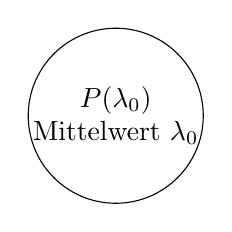
\begin{tikzpicture}[every text node part/.style={align=center}]
				\node[draw,circle,minimum size=1cm,inner sep=0pt] at (2,0) {$P(\lambda_0) $ \\ Mittelwert $ \lambda_0 $};
			\end{tikzpicture} & 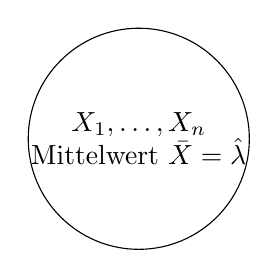
\begin{tikzpicture}[every text node part/.style={align=center}]
			\node[draw,circle,minimum size=1cm,inner sep=0pt] at (2,0) {$ X_1,\ldots,X_n $ \\ Mittelwert $ \bar{X} = \hat{\lambda} $};
		\end{tikzpicture}  \\
			$ \downarrow $ & $ \downarrow $ \\
			$ X_1,\ldots,X_n $ i.i.d. $ P(\lambda_0) $ & $ X_1^*,\ldots,X_n^* $ (ziehen mit Zurücklegen) \\
			$ \downarrow $ & $ \downarrow $ \\
			$ \bar{X} = \hat{\lambda} $ & $ \bar{X}^* = \hat{\lambda}^* $ \\
			\hline
			Fehler $ \hat{\lambda}-\lambda_0 $ & Fehler $ \hat{\lambda}^*-\hat{\lambda} $ \\
			\hline
			Wiederhole (u.a.), $ m $-mal: & Wiederhole (u.a.), $ m $-mal: \\
			$ \hat{\lambda}^{(1)}-\lambda_0,\ldots,\hat{\lambda}^{(m)}-\lambda_0 $ & $ \hat{\lambda}^{*(1)}-\hat{\lambda},\ldots,\hat{\lambda}^{*(m)}-\hat{\lambda} $ \\
			\hline
			$\F(t) = \Prob(\hat{\lambda}-\lambda_0) $ & $ \F(t) $ \\
			$ \approx $ Empirische Vfkt der $ \hat{\lambda}^{(i)} - \lambda_0, 1\le i\le m $ & $ \approx $ Empirische Vfkt der $ \hat{\lambda}^{*(i)} - \hat{\lambda}, 1\le i\le m $ \\
				& an der Stelle $ t $.
		\end{tabular}
	\vspace{1cm} 
	
		$ 95\% $ Konfidenzintervall mit der Bootstrap-Methode in R: 
		\[
		95\% \text{ CI } \left[ 8.206302,\; 8.532720 \right] 
		\]
		

	
\end{example}



\section{Parametrische Modelle und Parameterschätzung}
		\label{parameterschaetzung}

	\index{Parametrisches Modell}

\begin{itemize}
	\item Experiment:
\end{itemize}
Beobachtungen $ X_1,\ldots,X_n $\\

\begin{itemize}
	\item Modell:
\end{itemize}
Angenommen die $ X_1,\ldots,X_n $ sind i.i.d. Beobachtung einer Zufallsvariable $ X $, deren 
Verteilung von einer bestimmten Form ist:
	\[
	X\sim \; \text{Verteilung abhängig von einem Parameter} \; \theta_0 \in \Theta \subseteq \R^p
	\]
	
Die funktionale Form des Modells ist \underline{bekannt}, der Parameter $ \theta_0 $ ist \underline{unbekannt}!

\begin{example}
	Beispiele von parametrischen Modellen: \\
	
	
	\begin{tabular}{l|l}
			$ X\sim P(\lambda_0) $ 	& $ \lambda_0 = \theta_0 $ 				 \\
									& $ \Theta = \left(0,\infty\right) $ 	\\
			\midrule
			$ X\sim B(p_0) $		& $ p_0= \theta_0 $							\\
									& $ \Theta = \left(0,1\right) $ bzw. $ \left[0,1\right] $  \\
			\midrule
			$ X\sim \Bin(n,p)  $	& $ p_0= \theta_0 $						\\
			& $ \Theta = \left(0,1\right) $ bzw. $ \left[0,1\right] $  \\	
			\midrule
			$ X \sim N(\mu,\sigma_0^2) $ & $ \sigma_0^2 = \theta_0 $	 \\
									& $ \Theta = \left(0,\infty\right) $ bzw. $ [0,\infty) $  \\
			\midrule
			$ X \sim N(\mu_0,\sigma^2) $ & $ \mu_0 = \theta_0 $  \\
			& $ \Theta = \R $  \\
			\midrule
			$ X \sim N(\mu_0,\sigma_0^2) $ & $ \begin{pmatrix}
				\mu_0 \\ \sigma_0^2
			\end{pmatrix}\ = \theta_0 \; \ldots $ 2-dim.	 \\
			& $ \Theta = \R \times (0,\infty) $   		
		\end{tabular}

\end{example}

\begin{remark}
	Betrachte einen Schätzer $ \hat{\theta}_0 $ für $ \theta_0 $; das ist eine Größe $ \hat{\theta}=\hat{\theta} \left(X_1,\ldots,X_n \right) $, die alleine aus den Daten $ X_1, \ldots, X_n $ berechenbar ist (oft auch $ \hat{\theta}_n $). \\
	
	Beachte: Für $ \theta_0 \in \R^p $ mit $ p>1 $ ist auch $ \hat{\theta} \in \R^p $.
\end{remark}

\begin{definition}[Unverzerrtheit]
	\index{Unverzerrtheit}
	
	Der Schätzer $ \hat{\theta} $ für $ \theta_0 $ ist unverzerrt (bzw. erwartungstreu), wenn gilt: 
	\[
	\forall \theta \in \Theta: \tikzmarknode{E}{\E_\theta}\left(\hat{\theta}\right) = \theta.
	\]
	
	\begin{tikzpicture}[overlay, remember picture,shorten <=1mm,
	nodes={inner sep=1pt, align=center, font=\footnotesize}]
	\draw[<-] (E.south) -- ++ (0,-.5) node[below] {Erwartungstreu, wenn $ \theta $ \\ der wahre Parameter ist.};
	\end{tikzpicture}
	\vspace{1cm}

\end{definition}

\begin{remark} Beachte:
	Für $ \hat{\theta} = \begin{pmatrix}
		\hat{\theta}_1 \\ \vdots \\ \hat{\theta}_p
	\end{pmatrix} $ ist $ \E_\theta \left(\hat{\theta}\right) = \begin{pmatrix}
	 \E_\theta \left(\hat{\theta}_1\right) \\ \vdots \\  \E_\theta \left(\hat{\theta}_p\right)
\end{pmatrix} $. \\
Ist $ \hat{\theta} $ unverzerrt, dann ist die $ i $-te Komponente von $ \hat{\theta} $ ein unverzerrter Schätzer für die $ i $-te Komponente von $ \theta_0 $.
\end{remark}

\begin{definition}[Konsistenz]
	\index{Konsistenz}
	
	Ein Schätzer $  \hat{\theta}_{\tikzmarknode{n}{n}} $ für $ \theta_0 $ heißt konsistent, wenn gilt:
	
	\begin{tikzpicture}[overlay, remember picture,shorten <=1mm,
		nodes={inner sep=1pt, align=center, font=\footnotesize}]
		\draw[<-] (n.south) -- ++ (0,-.5) node[below] {Stichprobengröße};
	\end{tikzpicture}
	\vspace{1cm}
	
	\[
	\forall \epsilon > 0, \forall \theta \in \Theta : \Prob_\theta \left(||\hat{\theta}_n - \theta || > \epsilon \right) \overset{n\to\infty}{\longrightarrow} 0.
	\]
	
	Kurz: \[\hat{\theta}_n \overset{p}{\rightarrow}\theta_0.\]
\end{definition}

\begin{remark}
	Beachte: $ \hat{\theta}_n $ ist konsistent für $ \theta_0 $ genau dann, wenn $ \left(\hat{\theta}_n\right)_i $ konsistent ist für $ \left(\theta_0\right)_i $ für alle $ i=1,\ldots,p $.
\end{remark}

\begin{proof}[Nachrechnen]
	Siehe Übung.
\end{proof}

\underline{Wunschliste für Schätzer:}
\begin{itemize}
	\item Unverzerrtheit $ \qquad \qquad \leftarrow $ keinen systematischen Fehler.
	\item Konsistenz $ \qquad \qquad \qquad \leftarrow $ Genauigkeit wächst mit $ n $.
	\item kleine Varianz
	\item Verteilung des $ \hat{\theta}-\theta_0 $ bekannt oder approximierbar.
\end{itemize}

Zwei Strategien: 
\begin{itemize}
	\item Momentenmethode
	\item Maximum-Likelyhood-Methode.
\end{itemize}


\section{Die Momenten-Methode (MM)}

\begin{book}
 Siehe zu diesem Kapitel S. 260-267. in	\textit{Rice (2007)}.
\end{book}


Betrachte ein parametrisches Modell wie in Abschnitt \ref{parameterschaetzung}:
$ X_1,\ldots,X_n $ i.i.d. Kopien von $ X $, wobei $ X \sim $ Verteilung abhängig von $ \theta_0 \in \Theta \subseteq \R^p \quad (p\ge1) $.

In vielen Fällen gibt es eine eindeutige Beziehung zwischen dem Parameter $ \theta $ und einigen Momenten von $ X \quad (1:1) $.

\begin{example}
	
	
	\begin{tabular}{l|ll}
								& Parameter 	& Funktionen von $ \E(X), \E(X^2),\ldots $ \\
		\midrule
		$ X\sim P_\lambda $ 	& $ \lambda	$	& $ = \E(X) $\\
		\midrule
		$ X\sim B(n,p) $ 		& $ p $			& $ = \frac{1}{n} \E(X) $\\
		\midrule
		$ X\sim N(\mu, \sigma^2) $ & $ \mu $	& $ = \E(X) $\\
								& $ \sigma^2 $	& $ = \E(X^2)-(\E(X))^2 $
	\end{tabular}
\end{example}

	\begin{remark}
		(MM) Allgemein:
	
		Für $ \theta \in \Theta $ schreibt man 
		\[
		\E_\theta(X^k) = m_k(\theta) \qquad (=m_k)
		\]
		für $ k\ge1 $. Es gelte: 
		\[
		\theta = \begin{pmatrix}
			\theta_1 \\ \vdots \\ \theta_p
		\end{pmatrix} = f\left(m_1,\ldots,m_p\right)
		\]
		für eine Funktion $ f $, die geeignet glatt ist.
		
	\end{remark}

\index{Schätzer!Momenten-Methode}

Einen \textbf{Momenten-Methoden-Schätzer} \index{Momenten-Methoden-Schätzer} für $ \theta_0 $ erhält man nun folgendermaßen: 
	\begin{itemize}
		\item Schätze $ m_k $ durch \[ \hat{m}_k = \frac{1}{n} \sum_{i=1}^{n} X_i^k \] für $ k=1,\ldots,p $.
		\item Schätze $ \theta_0 $ durch \[\hat{\theta} = {\hat{\theta}}_{MM} = f\left(\hat{m}_1,\ldots,\hat{m}_p \right). \]
	\end{itemize}

\begin{remark}
	Bemerkung: Es gibt im Allgemeinem mehrere MM-Schätzer.
\end{remark}

\begin{example}[Gleichverteilung]
	$ X_1, \ldots, X_n $ i.i.d. $ U([0,\theta]), \; \theta > 0 $.
	
	\[
	\begin{aligned}
		\E(X_1) &= \frac{\theta}{2} & \Rightarrow \theta & = 2\E\left(X_1\right) \\
		& & \hat{\theta} & = 2 \frac{1}{n} \sum_{i=1}^{n} X_i. \\
		E(X_1^2) &= \frac{\theta^2}{3} & \Rightarrow \theta & = \sqrt{3\E\left(X_1^2\right)} \\
		& & \tilde{\theta} & = \sqrt{3\frac{1}{n} \sum_{i=1}^{n} X_i^2}. \\
		E(X_1^3) &= \ldots & \Rightarrow \ldots \\
		& & \ldots
	\end{aligned}
	\]
	
\end{example}


\begin{lemma}
	\label{lemma_stetig}
	Sind $ X_1,X_2,\ldots $ i.i.d. mit $ \E(X_1^k) = m_k $ für $ k = 1,\ldots, p $ und ist $ g:\R^p \rightarrow \R $ stetig im Punkt $ \left(m_1, \ldots, m_p \right) = m $, dann gilt für jedes $ \epsilon > 0 $
	\[
	\Prob\left(\left(g\left(\hat{m}_1,\ldots,\hat{m}_p\right)-g\left(m_1,\ldots,m_p\right)\right) > \epsilon \right) \overset{n\to\infty}{\longrightarrow} 0.
	\]
	(Hier ist $ \hat{m}_k = \frac{1}{n} \sum_{i=1}^{n} X_i^k $.)
\end{lemma}


\begin{remark}
	\index{Stetigkeit}
	Erinnerung:
	$ g: \R \rightarrow \R $ ist \textbf{stetig} im Punkt $ m \in \R $, wenn gilt: 
	\[ \forall \epsilon > 0 \; \exists \, \delta >0 \colon |m^\prime - m| < \delta \Rightarrow |g(m^\prime) - g(m)| < \epsilon. \]
	$ g: \R^p \rightarrow \R $ ist \textbf{stetig} im Punkt $ m \in \R^p $, wenn gilt: 
	\[ \forall \epsilon > 0 \; \exists \, \delta >0 \colon ||m^\prime - m|| < \delta \Rightarrow |g(m^\prime) - g(m)| < \epsilon. \]
\end{remark}


\begin{proof}
	Sei $ \epsilon > 0 $. Weil $ g $ stetig ist im Punkt $ m $, gibt es ein $ \delta > 0 $, sodass gilt: 
	\[ ||m^\prime - m|| < \delta \Rightarrow |g(m^\prime) - g(m)| < \epsilon. \]
	Setze $ \hat{m} = \begin{pmatrix}
		\hat{m}_1 \\ \vdots \\ \hat{m}_p
	\end{pmatrix} $. Dann gilt:

	\[
	\begin{aligned}
		\; & \left\lbrace||\hat{m} - m|| < \delta \right\rbrace & \subseteq & \left\lbrace|g(\hat{m}) - g(m)| < \epsilon \right\rbrace \\
		\Rightarrow	& \left\lbrace|g(\hat{m}) - g(m)| \ge \epsilon \right\rbrace & \subseteq & \left\lbrace||\hat{m} - m|| \ge \delta \right\rbrace
	\end{aligned}
	\]
	
	Also: 
	\[
	\begin{aligned}
		\Prob\left(|g(\hat{m})-g(m)|>\epsilon \right) & \le \Prob\left(|g(\hat{m})-g(m)|\ge\epsilon \right) \\
		& \le \Prob\left(||\hat{m}-m||\ge \delta \right) \\
		& \le \Prob\left(||\hat{m}-m||> \frac{\delta}{2} \right).
	\end{aligned}
	\]
	
	Mit dem Gesetz der großen Zahlen gilt: 
	\[
	\hat{m}_k = \frac{1}{n} \sum_{i=1}^{n} X_i^k \overset{p}{\longrightarrow} m_k \tag{$\hexstar\hexstar$}
	\]
	für jedes $ k=1,\ldots, p $. 
	
	\[
	\begin{aligned}
		\Prob\left(||\hat{m}-m||> \frac{\delta}{2} \right) & = \Prob\left(\sqrt{\sum_{k=1}^{p}\left(\hat{m}_k-m_k\right)^2} > \frac{\delta}{2} \right) \\
		& = \Prob\left(\sum_{k=1}^{p}\left(\hat{m}_k-m_k\right)^2 > \frac{\delta^2}{4} \right) \\
		& \overset{(\hexstar)}{\le} \sum_{k=1}^{p} \Prob\left(\left(\hat{m}_k-m_k\right)^2 > \frac{\delta^2}{4p} \right) \\
		& = \sum_{k=1}^{p} \underbrace{\Prob\left(\left|\hat{m}_k-m_k\right| > \frac{\delta}{2\sqrt{p}} \right)}_{\overset{n\to\infty}{\longrightarrow} 0 \, \text{wegen} \, (\hexstar\hexstar)} \\
		& \overset{n\to \infty}{\longrightarrow} 0. 		
	\end{aligned}
	\]
\end{proof}


\begin{remark}
	Bemerkung: Zu $ (\hexstar) $
	\begin{itemize}
		\item $ \Prob(A+B>\epsilon)\le \Prob\left(A>\frac{\epsilon}{2} \right) + \Prob \left(B > \frac{\epsilon}{2} \right), \; \text{denn:} $
		\[ \left\lbrace A \le \frac{\epsilon}{2} \right\rbrace \cap \left\lbrace B \le \frac{\epsilon}{2} \right\rbrace \subseteq \left\lbrace A +B \le \epsilon \right\rbrace\]
		
		\[ \left\lbrace A +B > \epsilon \right\rbrace \subseteq \left\lbrace A > \frac{\epsilon}{2} \right\rbrace \cup \left\lbrace B > \frac{\epsilon}{2} \right\rbrace \]
		
		\[ \begin{aligned}\Prob\left( A +B > \epsilon \right) & \le \Prob \left(\left\lbrace A > \frac{\epsilon}{2} \right\rbrace \cup \left\lbrace B > \frac{\epsilon}{2} \right\rbrace \right) \\
		 & \le \Prob\left(A>\frac{\epsilon}{2}\right) + \Prob\left(B>\frac{\epsilon}{2}\right).
		 \end{aligned}\]
		
		\item $ \Prob(A_1 + \ldots + A_p >\epsilon)\le \sum_{k=1}^{p} \Prob\left(A_k >\frac{\epsilon}{p} \right) \; \ldots \; \text{Übung.} $
	\end{itemize}
\end{remark}


\begin{satz}
	Betrachte $ X_i, \, i\ge 1, $ i.i.d. wie in (MM).
	
	Ist die Funktion $ f:\R^p \rightarrow \R^p $ stetig in jedem Punkt der Menge $ \left\lbrace \tikzmarknode{M}{\left(m_1(\theta),\ldots,m_p(\theta)\right)}^\prime = \theta \in \tikzmarknode{T}{\Theta} \right\rbrace $, dann ist $ \hat{\theta}_{MM} $ konsistent für $ \theta_0 $.
	
	\begin{tikzpicture}[overlay, remember picture,shorten <=1mm,
		nodes={inner sep=1pt, align=center, font=\footnotesize}]
		\draw[<-] (M.south) -- ++ (-0.5,-0.5) node[below] {alle möglichen Werte \\ der Momente}; 
		\draw[<-] (T.south) -- ++ (0.5,-0.7) node[below] {alle möglichen Werte \\ des Parameters}; 
	\end{tikzpicture}
	\vspace{1cm}
	
\end{satz}

\begin{proof}
	Sei $ \hat{\theta}_n $ der MM-Schätzer zur Stichprobengröße $ n $. 
	
	Zu zeigen: Für jede Komponente $ i = 1, \ldots, p $, gilt 
	\[ \forall \epsilon > 0 \; \forall \theta \in \Theta \quad \lim_{n\to \infty} \Prob_\theta \left( \left| \hat{\theta}_{n,i} - \theta_i \right| > \epsilon \right) = 0. \tag{$\hexstar$} \]
	
	$ \theta = f(m), \; \theta_i = f(m)_i $.
	
	Beachte: $ f(\cdot)_i \colon \R^p \rightarrow \R $ ist stetig, weil $ f \colon \R^p \rightarrow \R^p $ stetig ist. 
	
	Verwende Lemma \ref{lemma_stetig} mit $ f(\cdot)_i $ statt $ g $. Man erhält 
	\[
	\lim_{n\to \infty} \Prob_\theta (| \underbrace{f(\hat{m})_i}_{=\hat{\theta}_{n,i}} - \underbrace{f(m_i)}_{=\theta_{i}} | > \epsilon ) = 0.
	\]
	Also gilt $ (\hexstar) $.
\end{proof}


\begin{example}[Poissonverteilung]
	
	
	$ X_1, \ldots, X_n $ i.i.d. $ P(\lambda_0), \quad \lambda_0 > 0 $. 
	
	Beachte $ \E(X_1) = \lambda_0 $, sodass auch $ \E(\hat{\lambda}) = \lambda_0 $.
	
	MM-Schätzer: \[ \hat{\lambda} = \frac{1}{n} \sum_{i=1}^{n} X_i. \]
	
	Wissen: 
	
	$ \hat{\lambda} $ ist konsistent für $ \lambda_0. \checkmark $
	
	$ \hat{\lambda} $ ist unverzerrt. $ \checkmark $
\end{example}

\begin{example}[Normalverteilung]
	
	$ X_1, \ldots, X_n $ i.i.d. $ N\left(\mu_0, \sigma_0^2\right) $.
	
	$ \mu_0 = \E(X_1) $, 
	
	$ \sigma_0^2 = \E(X_1^2) - (\E(X_1))^2 $.
	
	MM-Schätzer: 
	\[
	\begin{pmatrix}
		\hat{\mu} \\ \hat{\sigma}^2 
	\end{pmatrix} 
	= \begin{pmatrix}
		\frac{1}{n} \sum_{i=1}^{n} X_i \\
		\frac{1}{n} \sum_{i=1}^{n} X_i^2 - \left(\frac{1}{n} \sum_{i=1}^{n} X_i\right)^2
	\end{pmatrix}.
	\]
	
	Die Funktion $ f \colon \R^2 \rightarrow \R^2, \; \begin{pmatrix} m_1 \\ m_2 \end{pmatrix} \mapsto \begin{pmatrix} m_1 \\ m_2-m_1^2 \end{pmatrix} $ ist stetig auf ganz $ \R^2 $. 
	
	Damit ist $ \begin{pmatrix} \hat{\mu} \\ \hat{\sigma}^2 \end{pmatrix} $ konsistent für $ \begin{pmatrix} \mu_0 \\ \sigma_0^2 \end{pmatrix} . \checkmark $
	
	$ \E(\hat{\mu}) = \E\left(\frac{1}{n} \sum_{i=1}^{n} X_i \right) = \E(X_1) = \mu_0 \; \ldots $ $ \hat{\mu} $ ist unverzerrt. $ \checkmark $
	
	$ \E(\hat{\sigma}^2): $ 
	
	\[
	\begin{aligned}
		\hat{\sigma}^2 & = \frac{1}{n} \sum_{i=1}^{n} X_i^2 - \left(\frac{1}{n} \sum_{i=1}^{n} X_i\right)^2 \\
		& = \frac{1}{n} \sum_{i=1}^{n} \left(X_i- \bar{X}_n \right)^2.
	\end{aligned}                      
	\]
	Aus der Vorlesung Grundzüge der Statistik wissen wir, dass 
	$ \E(\hat{\sigma}^2) = \frac{n-1}{n} \sigma^2 $. 
	
	$ \hat{\sigma}^2 $ ist also verzerrt. 
\end{example}


\begin{example}[Geometrische Verteilung]
	$ X_1, \ldots, X_n $ i.i.d. $ G(p_0), \quad p_0 \in (0,1) $.
	
	Wissen: Für $ X \sim G(p) $ ist 
	
	$ \E(X) = \frac{1}{p}, \quad \Rightarrow p = \frac{1}{\E(X)} $
	
	$ \Var(X) = \frac{1-p}{p^2} $.
	
	MM-Schätzer: 
	\[
	\hat{p}_n = \frac{1}{\bar{X}_n} = \frac{1}{\frac{1}{n} \sum_{i=1}^{n} X_i}.
	\]
	
	Die Funktion $ f(t) = \frac{1}{t} $ ist stetig auf $ (0,\infty) $. 
	
	Die Menge der möglichen Werte von $ \E_p(X_1) $ ist \[ \left\lbrace \E_p (X_1) \colon p\in (0,1) \right\rbrace = \left\lbrace \frac{1}{p} \colon 0<p<1 \right\rbrace = (0, \infty). \]
	
	Damit ist $ \hat{p}_n $ konsistent für $ p_0 . \checkmark $
	
	Erwartungstreue: 
	\[
	\begin{aligned}
		\E_p(\hat{p}_n)  & = \E_p \left( \frac{1}{\frac{1}{n}\sum_{i=1}^{n}X_i} \right) \\
		& \ne \frac{1}{\E_p\left(\frac{1}{n}\sum_{i=1}^{n}X_i \right) } = \frac{1}{\frac{1}{p}} = p.
	\end{aligned}
	\]
	Also ist der MM-Schätzer $ \hat{p}_n $ verzerrt.
\end{example}

\textbf{Verteilung des Schätzfehlers/Konfidenzintervalls:}

\begin{example}[Normalverteilung]
	$ X_1, \ldots, X_n $ i.i.d. $ N(\mu_0, \sigma_0^2) $. 
	
	
	\begin{itemize} \item Konfidenzintervall (KI) für $ \mu_0 $: \end{itemize}
	
	
	Wissen: \[\sqrt{n}\frac{\bar{X}_n-\mu_0}{\hat{\sigma}_n} \sim t_{n-1},\] 
	wobei $ \bar{X}_n = \frac{1}{n}\sum_{i=1}^{n} X_i = \hat{\mu}_{MM} $ und $ \tilde{\sigma}_n^2 = \frac{1}{n-1} \sum_{i=1}^{n} (X_i-\bar{X})^2 = \frac{n}{n-1}\hat{\sigma}_{MM}^2 $.
	
	Gegeben $ \alpha \in (0,1) $. Wähle $ a = \F_{t_{n-1}}^{-1} \left(\frac{\alpha}{2}\right) $ und $ b = \F_{t_{n-1}}^{-1} \left(1-\frac{\alpha}{2}\right) $ (Quantile der $ t_{n-1} $-Verteilung).
	
	Dann ist 
	\[
	\begin{aligned}
		\Prob\left(a\le\sqrt{n}\frac{\bar{X}_n-\mu_0}{\hat{\sigma}_n} \le b \right) & = \F_{t_{n-1}}(b) - \F_{t_{n-1}}(a) \\
		& = 1 - \frac{\alpha}{2} - \frac{\alpha}{2} \\
		& = 1 - \alpha.
	\end{aligned}
	\]
	
	\[
	\begin{aligned}
		\Prob\left(a\le\sqrt{n}\frac{\bar{X}_n-\mu_0}{\hat{\sigma}_n} \le b \right) & = \Prob\left(\frac{\hat{\sigma}_n}{\sqrt{n}}a \le \bar{X}_n - \mu_0 \le \frac{\hat{\sigma}_n}{\sqrt{n}}b \right) \\
		& = \Prob\left(- \bar{X}_n + \frac{\hat{\sigma}_n}{\sqrt{n}}a \le - \mu_0 \le - \bar{X}_n + \frac{\hat{\sigma}_n}{\sqrt{n}}b \right) \\
		& = \Prob\left(\bar{X}_n - \frac{\hat{\sigma}_n}{\sqrt{n}}a \ge \mu_0 \ge \bar{X}_n - \frac{\hat{\sigma}_n}{\sqrt{n}}b \right) \\
		& = \Prob\left(\bar{X}_n - \frac{\hat{\sigma}_n}{\sqrt{n}}b \le \mu_0 \le \bar{X}_n - \frac{\hat{\sigma}_n}{\sqrt{n}}a \right).
	\end{aligned}
	\]
	Also: Das KI $ \left[\bar{X}_n-\frac{\hat{\sigma}_n}{\sqrt{n}}b, \bar{X}_n-\frac{\hat{\sigma}_n}{\sqrt{n}}a \right] $ hat Überdeckungswahrscheinlichkeit $ 1-\alpha $.
	
	
	\begin{itemize} \item KI für $ \sigma_0^2 $: \end{itemize}
	
	Wissen: 
	\[
	\begin{aligned} 
		\sum_{i=1}^{n} (X_i-\bar{X}_n)^2 & \sim \sigma_0^2 \chi_{n-1}^2 \\
		\hat{\sigma}_n^2 & \sim \frac{\sigma_0^2 \chi_{n-1}^2}{n-1} \\
		(n-1) \frac{\hat{\sigma}_n^2}{\sigma_0^2} & \sim \chi_{n-1}^2 .
	\end{aligned}
	\]
	
	Gegeben $ \alpha \in (0,1) $  wählt man hier $ a = \F_{\chi_{n-1}^2}^{-1} \left(\frac{\alpha}{2}\right) $ und $ b = \F_{\chi_{n-1}^2}^{-1} \left(1-\frac{\alpha}{2}\right) $ (Quantile der $ \chi_{n-1}^2 $-Verteilung).
	
	Damit ist 
	\[
	\begin{aligned}
		\Prob\left(a\le (n-1) \frac{\hat{\sigma}_n^2}{\sigma_0^2} \le b \right) & = \F_{\chi_{n-1}^2}(b) - \F_{\chi_{n-1}^2}(a) \\
		& = 1 - \frac{\alpha}{2} - \frac{\alpha}{2} \\
		& = 1 - \alpha.
	\end{aligned}
	\]
	
	\[
	\begin{aligned}
		\Prob\left(a \le (n-1) \frac{\hat{\sigma}_n^2}{\sigma_0^2} \le b \right) & = \Prob\left(\frac{a}{(n-1)\hat{\sigma}_n^2} \le \frac{1}{\sigma_0^2} \le \frac{b}{(n-1)\hat{\sigma}_n^2} \right) \\
		& = \Prob\left(\frac{(n-1)\hat{\sigma}_n^2}{a} \ge \sigma_0^2 \ge \frac{(n-1)\hat{\sigma}_n^2}{b} \right)\\
		& = \Prob\left(\frac{(n-1)\hat{\sigma}_n^2}{b} \le \sigma_0^2 \le \frac{(n-1)\hat{\sigma}_n^2}{a} \right).
	\end{aligned}
	\]
	Also: Das KI $ \left[\frac{(n-1)\hat{\sigma}_n^2}{b}, \frac{(n-1)\hat{\sigma}_n^2}{a} \right] $ für $ \sigma_0^2 $ hat Überdeckungswahrscheinlichkeit $ 1-\alpha $.
\end{example}


\begin{example}[Poisson-Modell]
	$ X_1,\ldots,X_n $ i.i.d. $ P(\lambda_0), \quad (\lambda_0 > 0) $. 
	
	Hier ist $ \E(X_1)=\lambda_0, \quad \Var(X_1)=\lambda_0 $. 
	
	
	$ (\hexstar) $ \textit{Erinnerung aus der Vorlesung Grundzüge der Statistik:} 
	Für $ Z_1,\ldots, Z_n $ i.i.d. mit $ \E(Z_1) = \mu $ und $ \Var(Z_1) = \sigma^2 $. Ist ein KI für $ \mu $ mit \textbf{nominaler} \index{Konfidenzinterval!nominal} Überdeckungswahrscheinlichkeit $ 1 - \alpha $ 
	\[
	\left[\tilde{\mu} - \frac{\tilde{\sigma}}{\sqrt{n}} \Phi^{-1}\left(1-\frac{\alpha}{2}\right), \tilde{\mu} - \frac{\tilde{\sigma}}{\sqrt{n}} \Phi^{-1}\left(\frac{\alpha}{2}\right) \right]
	\]
	wobei $ \tilde{\mu}= \frac{1}{n}\sum_{i=1}^{n} Z_i $ und $ \tilde{\sigma}^2 = \frac{1}{n-1} \sum_{i=1}^{n} (Z_i - \tilde{\mu})^2 $.
	
	Zurück zum Beispiel: Für $ \lambda_0 $ ergibt das ein Ki mit nominaler Überdeckungswahrscheinlichkeit $ 1 - \alpha $: 
	\[
	\left[\bar{X}_n - \frac{\hat{\sigma}_n}{\sqrt{n}} \Phi^{-1}\left(1-\frac{\alpha}{2}\right), \bar{X}_n - \frac{\hat{\sigma}_n}{\sqrt{n}} \Phi^{-1}\left(\frac{\alpha}{2}\right) \right]
	\]
	wobei $ \hat{\sigma}_n^2 = \frac{1}{n-1} \sum_{i=1}^{n} (X_i - \bar{X}_n)^2 $ ein Schätzer für $ \Var(X_1) = \lambda_0 $ ist. Ein anderer Schätzer für $ \lambda_0 = \E(X_1) $ ist $ \bar{X}_n $.
	
	
	Im Kontext von $ (\hexstar) $ gilt (Siehe VO GZ: Beispiel 8.8): 
	
	\[
	\sqrt{n} \frac{\tilde{\mu}_n-\mu}{\sigma} \overset{w}{\longrightarrow} N(0,1), 
	\] und auch
	\[
	\sqrt{n} \frac{\tilde{\mu}-\mu}{\tilde{\sigma}_n} \overset{w}{\longrightarrow} N(0,1). 
	\]
	Betrachte einen anderen Varianzschätzer $ \check{\sigma}_n^2 $ für $ \sigma $ der konsistent ist: \[ \check{\sigma}_n^2 \xrightarrow{p} \sigma^2 . \]
	
	\[
	\sqrt{n} \frac{\tilde{\mu}_n - \mu}{\check{\sigma}_n} = \sqrt{n} \underbrace{\frac{\tilde{\mu}_n - \mu}{\sigma}}_{\xrightarrow{w}N(0,1)} \underbrace{\frac{\sigma}{\check{\sigma}_n}}_{\substack{ f(\check{\sigma}_n) \xrightarrow{p}1 \\ \text{ für } f(x) = \frac{\sigma}{x}.}} \xrightarrow{w} N(0,1)\cdot 1 \equiv N(0,1).
	\]
	Wissen: \[ \check{\sigma}_n^2 \xrightarrow{p} \sigma^2 \Rightarrow \check{\sigma}_n \xrightarrow{p} \sigma \Rightarrow \underbrace{f(\check{\sigma}_n)}_{=\frac{\sigma}{\check{\sigma}_n}} \xrightarrow{p} \underbrace{f(\sigma)}_{= \frac{\sigma}{\sigma}=1} \]
	
	
	Im Poisson-Modell ist $ \bar{X}_n $ ein konsistenter Schätzer für $ \E(X_1) = \lambda_0 $. Damit ist $ \bar{X}_n $ auch konsistent für $ \Var(X_1) = \lambda_0 $. 
	
	Damit gilt: 
	\[
	\sqrt{n} \frac{\bar{X}_n-\lambda_0}{\sqrt{\bar{X}_n}} \overset{w}{\longrightarrow} N(0,1). \tag{$\hexstar\hexstar$}
	\]
	
	Gegeben $ \alpha \in (0,1) $ wähle hier $ a = \Phi^{-1} \left(\frac{\alpha}{2}\right) $ und $ b = \Phi^{-1} \left( 1 - \frac{\alpha}{2} \right) $. 
	
	Dann ist 
	\[
	\begin{aligned}
		\Prob\left(a \le \sqrt{n} \frac{\bar{X}_n - \lambda_0}{\sqrt{\bar{X}_n}} \le b \right) & \overset{(\hexstar\hexstar)}{=} \Prob\left(\sqrt{n} \frac{\bar{X}_n - \lambda_0}{\sqrt{\bar{X}_n}} \le b \right) - \Prob\left(\sqrt{n} \frac{\bar{X}_n - \lambda_0}{\sqrt{\bar{X}_n}} \le a \right) \\
		& \approx \Phi (b) - \Phi (a) \\
		& = 1 - \frac{\alpha}{2} - \frac{\alpha}{2} \\
		& = 1 - \alpha.
	\end{aligned}
	\]
	
	\[
	\begin{aligned}
		\Prob\left(a \le \sqrt{n} \frac{\bar{X}_n - \lambda_0}{\sqrt{\bar{X}_n}} \le b \right) & = \Prob \left(\sqrt{\frac{\bar{X}_n}{n}} a \le \bar{X}_n - \lambda_0 \le \sqrt{\frac{\bar{X}_n}{n}} b \right) \\
		& = \Prob \left(- \bar{X}_n + \sqrt{\frac{\bar{X}_n}{n}} a \le  - \lambda_0 \le - \bar{X}_n + \sqrt{\frac{\bar{X}_n}{n}} b \right) \\
		& = \Prob \left(\bar{X}_n - \sqrt{\frac{\bar{X}_n}{n}} a \ge   \lambda_0 \ge  \bar{X}_n - \sqrt{\frac{\bar{X}_n}{n}} b \right) \\
		& = \Prob \left(\bar{X}_n - \sqrt{\frac{\bar{X}_n}{n}} b \le   \lambda_0 \le  \bar{X}_n - \sqrt{\frac{\bar{X}_n}{n}} a \right).
	\end{aligned}
	\]
	Also ist $ \left[\bar{X}_n - \sqrt{\frac{\bar{X}_n}{n}} b, \bar{X}_n - \sqrt{\frac{\bar{X}_n}{n}} a \right] $ ein KI für $ \lambda_0 $ mit nominaler Überdeckungswahrscheinlichkeit $ 1-\alpha $. 
	
	\begin{itemize}
		\item Spezielles Intervall im Poisson-Modell: 
		\[
		\left[\bar{X}_n - \sqrt{\frac{\bar{X}_n}{n}} b, \bar{X}_n - \sqrt{\frac{\bar{X}_n}{n}} a \right]
		\]
		
		\item Generisches Intervall: 
		\[
		\left[\bar{X}_n - \sqrt{\frac{\hat{\sigma}_n^2}{n}} \underbrace{\Phi^{-1}\left(1-\frac{\alpha}{2}\right)}_{=b}, \bar{X}_n - \sqrt{ \frac{\hat{\sigma}_n^2}{n}} \underbrace{\Phi^{-1}\left(\frac{\alpha}{2}\right)}_{=a} \right]
		\]
	\end{itemize}
	
\end{example}

\begin{example}[Geometrische Verteilung]
	$ X_1, \ldots, X_n \sim G(p_0), \quad p_0 \in (0,1) $. 
	
	Wissen: $ \E(X_1) = \frac{1}{p_0}, \quad \Var(X_1) = \frac{1-p_0}{p_0^2} $, MM-Schätzer $ \hat{p}_n = \frac{1}{\bar{X}_n} $ (nicht linear!).
	
	Hinweis zur geometrischen Verteilung: 
	\begin{itemize}
	\item $ \# $ Versuche bis zum 1. Erfolg (wird in der Vorlesung verwendet)
	\item $ \# $ Misserfolge bis zum 1. Erfolg + 1 (wird in R verwendet).
	\end{itemize}

	Setze $ \mu_0 = \E(X_1) = \frac{1}{p_0} $. Mit zentralem Grenzwertsatz gilt: 
	\[
	\Prob\left(\sqrt{n} \frac{\bar{X}_n - \mu_0}{\sqrt{\frac{1-p_0}{p_0^2}}} < t \right) \xrightarrow{n\to\infty} \Phi(t).
	\]
	
	Also: Verteilung von $ \sqrt{n} \frac{\bar{X}_n - \mu_0}{\sqrt{\frac{1-p_0}{p_0^2}}} \xrightarrow{w} N(0,1) $.
	
%	Idee: \[
%	\begin{aligned}
%		\bar{X}_n & \approx N(\cdot,\cdot) \\
%		\alpha \bar{X}_n + \beta & \approx N(\cdot,\cdot).
%	\end{aligned}
%	\]
	
	
	Wissen:  $ \hat{p}_n = \frac{1}{\bar{X}_n} $, also der MM-Schätzer für $ p_0 $, ist konsistent. 
	
	D.h. $ \hat{p}_n \xrightarrow{p} p_0 $. 
	
	Die Funktion $ g(t) = \sqrt{\frac{1-t}{t^2}} $ ist stetig im Punkt $ p_0 \in (0,1) $. 
	
	\[ \Rightarrow f(\hat{p}_n) \xrightarrow{p} f(p_0), \] 
	
	d.h. \[ \sqrt{\frac{1-\hat{p}_n}{\hat{p}_n^2}} \xrightarrow{p} \sqrt{\frac{1-p_0}{p_0^2}}. \]
	
	Man erhält folgendes: 
	\[
	\begin{aligned}
		\sqrt{n}\frac{\bar{X}_n - \mu_0}{\sqrt{\frac{1-\hat{p}_n}{\hat{p}_n^2}}} & = \underbrace{\sqrt{n}\frac{\bar{X}_n - \mu_0}{\sqrt{\frac{1-p_0}{p_0^2}}}}_{\xrightarrow{w} N(0,1)} \underbrace{\frac{\tikzmarknode{Z}{\sqrt{\frac{1-p_0}{p_0^2}}}}{\tikzmarknode{N}{\sqrt{\frac{1-\hat{p}_n}{\hat{p}_n^2}}}}}_{\xrightarrow{p}1} \\
		& \tikzmarknode{K}{\xrightarrow{w}} N(0,1)\cdot 1 \equiv N(0,1).
	\end{aligned}
	\]
	
	\begin{tikzpicture}[overlay, remember picture,shorten <=1mm,
		nodes={inner sep=1pt, align=center, font=\footnotesize}]
		\draw[<-] (Z.east) -- ++ (1, 0.5) node[right] {Zähler fest}; 
		\draw[<-] (N.east) -- ++ (1, -0.5) node[right] {Nenner $\xrightarrow{p}$ Zähler}; 
		\draw[<-] (K.south) -- ++ (-0.5, -0.5) node[below] {(Siehe Rechenregeln für \\ $\xrightarrow{p}, \xrightarrow{w}$, GZS S. 80)};
	\end{tikzpicture}
	\vspace{1cm}
	
	Man erhält daraus, ähnlich wie im letzten Beispiel ein Konfidenzintervall für $ \mu_0 $, nämlich
	\[
	\left[ 
	\bar{X}_n - \sqrt{\frac{\frac{(1-\hat{p}_n)}{\hat{p}_n^2}}{n}} \Phi^{-1} \left(1-\frac{\alpha}{2}\right), \bar{X}_n - \sqrt{\frac{\frac{(1-\hat{p}_n)}{\hat{p}_n^2}}{n}} \Phi^{-1} \left(\frac{\alpha}{2}\right)\right], 
	\]
	mit nominaler Überdeckungswahrscheinlichkeit $ 1-\alpha $. 
	
	Aber: $ \mu_0 = \frac{1}{p_0} $, und gesucht ist ein Konfidenzintervall für $ p_0 = \frac{1}{\mu_0} $ (nicht-lineare Funktion von $ \mu_0 $). 
	
	Siehe Beispiel unten für Fortsetzung des Beispiels.
\end{example}

Lineare Funktionen von $ \mu_0 $ sind einfach zu berechnen: 

Angenommen man interessiert sich für $ \alpha\mu_0 + \beta, \quad \alpha \ne 0, \quad \beta \in \R $. 

Das ist einfach: \[\Prob\left(\hat{A} \le \mu_0 \le \hat{B}\right) \overset{\alpha > 0}{=} \Prob\left(\alpha\hat{A} + \beta \le \alpha \mu_0 + \beta \le \alpha \hat{B} + \beta\right). \]
Damit ist ein Konfidenzintervall für $ \alpha \mu_0 + \beta $ mit nominaler Überdeckungswahrscheinlichkeit $ 1-\alpha $ gegeben durch 
	\[
	\left[ \alpha \left(
	\bar{X}_n - \sqrt{\frac{\frac{(1-\hat{p}_n)}{\hat{p}_n^2}}{n}} \Phi^{-1} \left(1-\frac{\alpha}{2}\right)\right) + \beta, \alpha \left( \bar{X}_n - \sqrt{\frac{\frac{(1-\hat{p}_n)}{\hat{p}_n^2}}{n}} \Phi^{-1} \left(\frac{\alpha}{2}\right)\right) + \beta \right]. 
	\]

\begin{satz}[$\delta$-Methode]
	\index{Delta-Methode}
	
	Es seien $ Z_1,Z_2, \ldots $ i.i.d. Kopien von $ Z $, mit $ \E(Z) = \mu_Z $ und $ \Var(Z) = \sigma_Z^2 > 0 $. 
	
	Ist $ f\colon \R \rightarrow \R $ eine Funktion, die \textbf{differenzierbar} ist im Punkt $ \mu_Z $, dann gilt: 
	\[
	\sqrt{n}\left(f(\bar{Z}_n)-f(\mu_Z)\right) \xrightarrow{w} N\left(0, \left(f^\prime \left(\mu_Z\right)\right)^2 \sigma_Z^2 \right), 
	\]
	wobei $ \bar{Z}_n = \frac{1}{n}\sum_{i=1}^{n}Z_i $.
\end{satz}

Illustration: Siehe R-script vom 22.04.2021.

\begin{proof}
	
	Erinnerung: 
	
	\begin{tabular}{l|l}
		$ \sqrt{n}\left(\bar{Z}_n - \mu_z \right) \xrightarrow{w} N(0, \sigma_Z^2) $ & Zentraler Grenzwertsatz \\
		\midrule
		$ \bar{Z}_n \xrightarrow{p} \mu_Z $ & Gesetz der großen Zahlen	\\
		\midrule
		$ X_n \xrightarrow{p} c, f(\cdot) $ stetig in $ c $ & Rechenregeln für $\xrightarrow{p}, \xrightarrow{w}$, GZS S. 80 \\
		$ \quad \Rightarrow f(X_n) \xrightarrow{p} f(c) $ & \\
		$ X_n \xrightarrow{w} X, Y_n \xrightarrow{p} c $ & \\
		$ \quad \Rightarrow X_n + Y_n \xrightarrow{w} X+c $ & \\
		$ \quad \Rightarrow X_n \cdot Y_n \xrightarrow{w} X\cdot c $ & \\
		\midrule
		$ f^\prime(\mu_Z) = \lim_{Z\to\mu_Z} \frac{f(Z)-f(\mu_Z)}{Z-\mu_z} $ & VO Analysis	
	\end{tabular}
	
	Definiere eine Funktion $ R(Z) $ als 
	\[
	R(Z)=\left\{\begin{array}{ll}
		f^\prime(\mu_z) - \frac{f(Z)-f(\mu_z)}{Z-\mu_Z} & \colon Z \ne Z_0, \\
		0 & \colon Z = \mu_Z .
	\end{array}\right .
	\]
	
	Beachte: $ R(Z) $ ist stetig im Punkt $ Z= \mu_Z $: 
	\[
	\lim_{Z\to\mu_Z} R(Z) \tikzmarknode{D}{=} 0 \tikzmarknode{O}{=} R(\mu_Z).
	\]
	
	\begin{tikzpicture}[overlay, remember picture,shorten <=1mm,
		nodes={inner sep=1pt, align=center, font=\footnotesize}]
		\draw[<-] (D.south) -- ++ (-1, -1) node[below] {weil $ f $ differenzierbar \\ ist im Punkt $ \mu_Z $}; 
		\draw[<-] (O.south) -- ++ (1, -1) node[below] {siehe \\ oben}; 
	\end{tikzpicture}
	\vspace{2cm}
	
	Dann gilt für $ Z \ne \mu_Z $: 
	
	\[
	\begin{aligned}
		&& f^\prime(\mu_Z) & = \frac{f(Z)-f(\mu_Z)}{Z-\mu_Z} + R(Z) \\
		&\Rightarrow & (Z-\mu_Z)f^\prime(\mu_Z) & = f(Z)-f(\mu_Z) + (Z-\mu_Z) R(Z) \\
		&\Rightarrow & \underbrace{f(Z)-f(\mu_Z)}_{\text{nicht-linear in } Z} & = \underbrace{f^\prime(\mu_Z)(Z-\mu_Z))}_{\text{linear in } Z} - \underbrace{(Z-\mu_Z)R(Z)}_{\text{Fehler}}.
	\end{aligned}
	\]
	
	Ersetze $ Z $ durch $ \bar{Z}_n $ und multipliziere mit $ \sqrt{n} $: 
	
	\[
	\begin{aligned}
		\sqrt{n} \left(f(\bar{Z}_n)-f(\mu_Z)\right) & = \underbrace{f^\prime(\mu_Z)\underbrace{\sqrt{n}\left(\bar{Z}_n-\mu_Z\right)}_{\xrightarrow{w}N(0,\sigma_Z^2)}}_{\xrightarrow{w}N\left(0,(f^\prime(\mu_Z))^2\sigma_Z^2\right)} - \underbrace{\underbrace{\sqrt{n}(\bar{Z}_n-\mu_Z)}_{\xrightarrow{w}N(0,\sigma_Z^2)}\underbrace{R(\bar{Z}_n)}_{\xrightarrow{p}R(\mu_Z)=0}}_{\xrightarrow{w}N(0,\sigma_Z^2)\cdot 0 = 0} \\
		&  \xrightarrow{w} N\left(0, (f^\prime(\mu_Z))^2\sigma_Z^2\right).
	\end{aligned}
	\]
	
\end{proof}


\begin{example}[Fortsetzung des oberen Beispiels - Geometrische Verteilung]
	
	$ X_i, \quad i \ge 1 $, i.i.d. $ G(p_0), \quad p_0 \in (0,1) $. 
	
	Wissen: \[ \bar{X}_n \xrightarrow{p} \frac{1}{p_0}, \quad \hat{p}_n = \frac{1}{\bar{X}_n} \xrightarrow{p} p_0 . 
	\]
	\[
	\sqrt{n}\left(\bar{X}_n-\frac{1}{p_0}\right) \xrightarrow{w} N\left(0, \frac{1-p_0}{p_0^2} \right) .
	\]
	
	Betrachte $ f(t) = \frac{1}{t} \ldots $ differenzierbar für $ t \ne 0 $ mit $ f^\prime(t) \overset{t\ne0}{=} - \frac{1}{t^2} $. 
	
	Weil $ p_0 \ne 0 $ ist, kann man die $ \delta $-Methode anwenden: 
	
	\[
	\begin{aligned}
	&& \sqrt{n}\left(f\left(\bar{X}_n\right) -f\left(\frac{1}{p_0}\right)\right) & \xrightarrow{w} N\left(0, \left(f^\prime \left(\frac{1}{p_0}\right)\right)^2 \frac{1-p_0}{p_0^2} \right) \\
	& \Rightarrow & \sqrt{n}\left(\frac{1}{\bar{X}_n} - \frac{1}{\frac{1}{p_0}}\right) & \xrightarrow{w} N\left(0, \left(-\frac{1}{\left(\frac{1}{p_0}\right)^2}\right)^2 \frac{1-p_0}{p_0^2} \right) \\
	& \Rightarrow & \sqrt{n}\left(\hat{p}_n - p_0 \right) & \xrightarrow{w} N\left(0, p_0^4\frac{1-p_0}{p_0^2} \right) \\
	& \Rightarrow & \sqrt{n}\left(\hat{p}_n-p_0\right) & \xrightarrow{w} N\left(0, p_0^2(1-p_0)\right).
	\end{aligned}
	\] 

	
	Damit erhält man ein Konfidenzintervall für $ p_0 $ wie folgt: 
	\[
	\sqrt{n}\frac{\hat{p}_n - p_0}{p_0\sqrt{1-p_0}} \xrightarrow{w} N(0,1).
	\]
	
	\[
	\begin{aligned}
	\sqrt{n}\frac{\hat{p}_n-p_0}{\hat{p}_n\sqrt{1-\hat{p}_n}} & = \underbrace{\sqrt{n}\frac{\hat{p}_n-p_0}{p_0\sqrt{1-p_0}}}_{\xrightarrow{w}N(0,1)} \underbrace{\frac{p_0\sqrt{1-p_0}}{\hat{p}_n\sqrt{1-\hat{p}_n}}}_{\xrightarrow{p}1} \\
	& \xrightarrow{w} N(0,1).
	\end{aligned}
	\]
	
	Für $ \alpha \in (0,1) $ ist ein Konfidenzintervall für $ p_0 $ mit nominaler Überdeckungswahrscheinlichkeit $ 1-\alpha $ damit gegeben durch 
	\[
	\left[ 
	\hat{p}_n - \sqrt{\frac{\hat{p}_n^2(1-\hat{p}_n)}{n}} \Phi^{-1} \left(1-\frac{\alpha}{2}\right), \hat{p}_n - \sqrt{\frac{\hat{p}_n^2(1-\hat{p}_n)}{n}} \Phi^{-1} \left(\frac{\alpha}{2}\right) \right] .
	\]
\end{example}

\begin{remark}
	Bemerkung:
	Das letzte Beispiel zeigt die Konstruktion von Konfidenzintervallen mit zentralem Grenzwertsatz und $ \delta $-Methode. Eine alternative Konstruktion liefert der Bootstrap.
\end{remark}

\begin{remark}
	Bemerkung:
	Es gibt auch eine multivariate Version der $ \delta $-Methode.
\end{remark}

Im letzten Beispiel ist die Überdeckungswahrscheinlichkeit des Konfidenzintervalls für $ p_0 $ nur nominal gleich $ 1-\alpha $. Wie groß ist die tatsächliche Überdeckungswahrscheinlichkeit dieses Konfidenzintervalls? Wie groß muss man $ n $ wählen, damit die tatsächliche 
Überdeckungs- wahrscheinlichkeit im Bereich $ 95\%\pm1 $ liegt (für $ \alpha = 0.05 $).


Simulation in R: \\


\begin{tabular}{l|ccccccc}
	$ n/p_0 $	& 5	& 20	& 80 	& 320	& 640 	& 1280 	& 2560 \\
	\midrule
	0.01		& $\checkmark$	& $\checkmark$	& $\checkmark$	& $\checkmark$	& $\checkmark$	& $\checkmark$	& $\checkmark$ \\
	0.1			& $\checkmark$	& $\checkmark$	& $\checkmark$	& $\checkmark$	& $\checkmark$	& $\checkmark$	& $\checkmark$ \\
	0.5			& $\times$	& $\checkmark$	& $\checkmark$	& $\checkmark$	& $\checkmark$	& $\checkmark$	& $\checkmark$ \\
	0.9			& $\times$	& $\times$	& $\times$	& $\checkmark$	& $\checkmark$	& $\checkmark$	& $\checkmark$ \\
	0.99		& $\times$	& $\times$	& $\times$	& $\times$	& $\times$	& $\times$	& $\checkmark$
\end{tabular}
\vspace{0.5cm}

Die Qualität der Approximation hängt von $ p_0 $ ab. 

Aber: $ p_0 $ ist konsistent schätzbar! 

Die Qualität der Approximation durch zentralen Grenzwertsatz und durch die $ \delta $-Methode ist $ p_0 $-abhängig: 
\[
\forall\; p_0 \colon \text{Fehler }(p_0) \xrightarrow{n\to\infty} 0,
\]
eine sogenannte \textbf{punktweise Approximation} \index{Approximation!punktweise}. In manchen Szenarien kann man eine sogenannte \textbf{gleichmäßige Approximation} \index{Approximation!gleichmäßige} finden. Für eine solche gilt:
\[
\underset{p_0}{\sup} \quad \text{Fehler }(p_0) \xrightarrow{n\to\infty} 0.
\]

Im geometrischem Modell ist eine solche gleichmäßige Approximation nicht verfügbar.


\section{Die Maximum-Likelihood Methode (ML)}

\begin{book}
	Siehe zu diesem Kapitel S. 267-285. in	\textit{Rice (2007)}.
\end{book}


Betrachte i.i.d. Zufallsvariablen $ X_1,\ldots,X_n $ deren jeweilige Dichte bzw. Wahrscheinlichkeitsfunktion von folgender Form ist: 
\[
f(x|\theta_0), \qquad \theta_0 \in \Theta \subseteq \R^p.
\]

Die funktionale Form von $ f(x|\theta_0) $ ist bekannt, aber der Parameter $ \theta_0 $ ist unbekannt. 

\begin{remark}
	Idee: Gegeben Beobachtungen $ x_1,\ldots,x_n $ von $ X_1,\ldots,X_n $ schätzt man $ \theta_0 $ durch jenen Wert von $ \theta\in\Theta $, für welchen die Beobachtungen ''am Wahrscheinlichsten'' sind. Man wählt also jenes $ \theta\in\Theta $, das die Beobachtungen ''am Besten beschreibt''. 
\end{remark}

	
\textbf{Diskrete Modelle:} \\

Diskrete Zufallsvariablen $ X_1,\ldots,X_n $, die i.i.d. sind mit Wahrscheinlichkeitsfunktion 
\[
p(x|\theta_0), \quad \theta_0\in\Theta, \quad x\in\N.
\]

Betrachte Beobachtungen $ x_1,\ldots,x_n $ von $ X_1,\ldots,X_n $. Ist der wahre Parameter gleich $ \theta\in\Theta $, dann ist die Wahrscheinlichkeit, die Werte $ x_1,\ldots,x_n $ zu beobachten, gegeben durch 
\[
p_\theta \left(X_1=x_1,X_2=x_2,\ldots,X_n=x_n\right) \coloneqq L(\theta).
\]

$ L(\theta) $ nennt man die \textbf{Likelihood}\index{Likelihood}. 

Beachte $ L(\theta) = p(x_1|\theta)\cdotp(x_2|\theta)\cdot\ldots\cdot p(x_n|\theta) $.

Alternativ dazu betrachtet man oft die sogenannte Log-Likelihood
\[\begin{aligned}
	l(\theta) & = \log(L(\theta)) \\
	& = \sum_{i=1}^{n}\log p(x_i|\theta).
\end{aligned}
\]

\begin{remark}
	Beachte: $ L(\theta) $ und $ l(\theta) $ hängen von den beobachteten Werten $ x_1,\ldots,x_n $ ab.
\end{remark}

Die Maximum-Likelihood Methode \index{Maximum-Likelihood Methode} maximiert $ L(\theta) $ über $ \theta\in\Theta $: \\
\[
\hat{\theta}_{ML} = \underset{\theta\in\Theta}{\operatorname{argmax}} \; L(\theta),
\]
wobei $ \hat{\theta}_{ML} $ ein Maximum-Likelihood-Schätzer für $ \theta $ ist. 

\begin{remark}
	Beachte: Ein Maximierer von $ L(\theta) $ ist auch ein Maximierer von $ l(\theta) $, und umgekehrt.
\end{remark}

\begin{remark}
	Bemerkung: Der Maximierer von $ L(\theta) $ (bzw. $ l(\theta) $) muss nicht eindeutig sein.
\end{remark}

\begin{example}[Bernoulli-Verteilung]
	$ X_1,\ldots,X_n $ i.i.d. $ B(\theta_0), \quad \theta_0 \in (0,1) $. Die Wahrscheinlichkeitsfunktion ist hier 
	\[
	\begin{aligned}
	p(x|\theta_0) & =\left\{\begin{array}{ll}
		\theta_0 & \colon x=1, \\
		1-\theta_0 & \colon x=0 \end{array}\right .\\
	& = \theta_0^x(1-\theta_0)^{1-x}.
	\end{aligned}
	\]
	
	Für Beobachtungen $ x_1,\ldots,x_n $ von $ X_1,\ldots,X_n $ ist die Likelihood gegeben durch 
	\[
	\begin{aligned}
		L(\theta) & = p(x_1|\theta)\cdot\ldots\cdot p(x_n|\theta) \\
		& = \underbrace{\left(\theta^{x_1}(1-\theta)^{1-x_1}\right)\left(\theta^{x_2}(1-\theta)^{1-x_2}\right)\cdot\ldots\cdot \left(\theta^{x_n}(1-\theta)^{1-x_n}\right)}_{n \text{ Faktoren. Jeder Faktor ist entweder gleich }\theta \text{ oder } 1-\theta} \\
		& = \theta^{\sum_{i=1}^{n}x_i}(1-\theta)^{n-\sum_{i=1}^{n}x_i} \\
		& = \theta^S (1-\theta)^{n-S}
	\end{aligned}
	\] 
	für $ S = \sum_{i=1}^{n}x_i $.
	
	\[
	\begin{aligned}
		l(\theta) & = \log\left(\theta^S(1-\theta)^{n-S}\right) \\
		& = S\cdot \log(\theta) + (n-S)\log(1-\theta).
	\end{aligned}
	\]
\vspace{0.5cm}	
	\[
	\begin{aligned}
		\frac{dl(\theta)}{d\theta} & = S \frac{1}{\theta} + (n-S)\frac{-1}{1-\theta} \\
		& = \frac{S}{\theta} -\frac{n-S}{1-\theta}.		
	\end{aligned}
	\]
\vspace{0.5cm}	
	\[
	\begin{aligned}
		&& \frac{dl(\theta)}{d\theta} & \overset{!}{=} 0 \\
		& \Leftrightarrow & \frac{S}{\theta} & = \frac{n-S}{1-\theta} \\
		& \Leftrightarrow & S(1-\theta) & = \theta (n-S) \\
		& \Leftrightarrow & S -S\theta & = n\theta - S\theta \\
		& \Leftrightarrow & \frac{S}{n} & = \theta_{\hexstar}.
	\end{aligned}
	\]
\vspace{0.5cm}	
	\[
	\begin{aligned}
		\frac{d^2l(\theta)}{d\theta^2} & = -\frac{S}{\theta^2} -(n-S)\frac{-1}{(1-\theta)^2}\\
		& = -\left(\frac{S}{\theta^2}+\frac{n-S}{(1-\theta)^2}\right). 
	\end{aligned}
	\]
	
	Wissen: \\
	
	$ S\in\lbrace0,1,\ldots,n\rbrace, $ sodass $ S \ge 0 $ \\
	
	$ n-S\in\lbrace0,1,\ldots,n\rbrace, $ sodass $ n-S \ge 0 $.\\
	
	$ \theta\in(0,1), $ sodass $ \theta > 0 $ \\
	
	$ 1-\theta\in(0,1), $ sodass $ 1-\theta > 0 $. \\
	
	$ \Rightarrow \frac{d^2l(\theta)}{d\theta^2} > 0 $, und $ \theta_{\hexstar} $ ist ein Maximierer.
	
	Also ist der ML-Schätzer für $ \theta_0 $ gegeben durch 
	\[
	\hat{\theta}_{ML} = \frac{S}{n} = \bar{x}_n \quad \ldots \quad \text{Stichprobenmittel}.
	\]
	
	Vor Beobachtungen der Daten ist der ML-Schätzer für $ \theta_0 $ die Zufallsvariable 
	\[
	\hat{\theta}_{ML} = \bar{X}_n.
	\]
	
	Beachte: $ \E_{\theta}(X_1)=\theta $. 
	
	Ein Momenten-Methoden Schätzer für $ \theta_0 $ ist damit gegeben durch $ \hat{\theta}_{MM} = \bar{X}_n $. Hier stimmen Maximum-Likelihood und Momentenmethode überein.
\end{example}


\textbf{Stetige Zufallsvariablen:}

Betrachte i.i.d. Zufallsvariablen $ X_1,\ldots,X_n $ mit Werten in $ \R $ und mit Dichte 
\[
f(x|\theta_0), \quad \theta_0\in\Theta
\]

Gegeben Beobachtungen $ x_1,\ldots,x_n $ von $ X_1,\ldots,X_n $ definiert man die \textbf{Likelihood} als 
\[
L(\theta) = f(x_1|\theta)\cdot f(x_2|\theta)\cdot\ldots\cdot f(x_n|\theta).
\]

\begin{remark}
	Bemerkung: Die Likelihood einer stetigen Zufallsvariable kann als Grenzfall der Likelihoods von diskreten Zufallsvariablen betrachtet werden. 
\end{remark}

Alternativ zu $ L(\theta) $ betrachtet man oft die Log-Likelihood 
\[
l(\theta) = \log L(\theta) = \sum_{i=1}^{n} \log f(x_i|\theta).
\]

\begin{remark}
	Bemerkung: $ L(\theta) $ und $ l(\theta) $ hängen von den Daten $ x_1,\ldots,x_n $ ab.
\end{remark}

Der Maximum-Likelihood Schätzer maximiert $ L(\theta) $ bzw. $ l(\theta) $ über $ \theta\in\Theta $: 

\[
\begin{aligned}
	\hat{\theta}_{ML} & = \underset{\theta\in\Theta}{\argmax}\; L(\theta) \\
	& = \underset{\theta\in\Theta}{\argmax}\; l(\theta) .
\end{aligned}
\]

\begin{remark}
	Bemerkung: Im Allgemeinem muss $ \hat{\theta}_{ML} $ nicht eindeutig sein.
\end{remark} 

\begin{example}[Exponentialverteilung]
	$ X_1,\ldots,X_n $ i.i.d. $ Exp(\lambda_0), \quad \lambda_0 >0 $. 
	
	D.h. $ \E(X_1)=\frac{1}{\lambda_0} $, und Dichte $ f(x|\lambda_0) = \lambda_0 e^{-\lambda_0 x} \quad (x\ge0) $.
	
	Für Beobachtungen $ x_1,\ldots,x_n $ ist 
	\[
	\begin{aligned}
		L(\theta) & = \prod_{i=1}^{n} f(x_i|\lambda) \\
		& = \prod_{i=1}^{n} \lambda e^{-\lambda x_i} \\
		& = \lambda^n e^{-\sum_{i=1}^{n}\lambda x_i} \\
		& = \lambda^n e^{-\lambda S}
	\end{aligned}
	\]
	für $ S = \sum_{i=1}^{n} x_i $.
	
	\[
	l(\lambda) = n \log \lambda - \lambda S.
	\]
	
	\[
	\begin{aligned}
		l^\prime (\lambda) & = \frac{n}{\lambda} - S &  \overset{!}{=} & 0 \\
		& \Leftrightarrow \frac{n}{\lambda} & = & S \\
		& \Leftrightarrow \frac{\lambda}{n} & = & \frac{1}{S} \\
		& \Leftrightarrow \lambda & = & \frac{1}{\frac{S}{n}} = \frac{1}{\bar{X}_n}.
	\end{aligned}
	\]
	
	\[
	l^{\prime\prime} (\lambda) = \frac{d}{d\lambda} \left(\frac{n}{\lambda} - S \right) = - \frac{n}{\lambda^2} < 0.
	\]
	
	Damit ist der Maximum-Likelihood-Schätzer für $ \lambda_0 $ gegeben durch 
	\[
	\hat{\lambda}_{ML} = \frac{1}{\bar{X}_n}.
	\]
\end{example}

\begin{remark}
	Beachte: Da $ \E(X_1)=\frac{1}{\lambda_0} $ ist, also $ \lambda_0 = \frac{1}{\E(X_1)} $, ist der Maximum-Likelihood-Schätzer für $ \lambda_0 $ auch ein Momentenmethoden-Schätzer.
\end{remark}

\begin{example}[Gleichverteiltes Skalenmodell]
	$ X_1,\ldots,X_n $ i.i.d. $ U([0,\theta_0]), \quad \theta_0 > 0 $. 
	
	Die Dichte von $ X_1 $ ist gegeben durch 
	\[
	f(x_1|\theta_0)=\left\{\begin{array}{ll}
		\frac{1}{\theta_0} & \colon 0\le x\le \theta_0, \\
		0 & \colon \text{sonst} .
	\end{array}\right .
	\]
	
	
	\[
	L(\theta) = \prod_{i=1}^{n} f(x_i|\theta)=\left\{\begin{array}{ll}
		\left(\frac{1}{\theta}\right)^n & \colon \underset{1\le i\le n}{\max(x_i)} \le \theta, \\
		0 & \colon \theta < \underset{1\le i\le n}{\max(x_i)} .
	\end{array}\right .
	\]
	Sei $ \underset{1\le i\le n}{\max(x_i)} = x_{(n)} $. 
	
	Achtung: $ L(\theta) $ ist nicht differenzierbar an der Stelle $ \theta = x_{(n)} $. 
	
	Weil $ \E(X_1) = \frac{\theta_0}{2} $, also $ \theta_0 = 2 \E (X_1) $, ist ein Momentenmethoden-Schätzer für $ \theta_0 $ gegeben durch $ \hat{\theta}_{MM} = 2 \bar{X}_n $.
	
	Hier ist $ \hat{\theta}_{ML} \ne \hat{\theta}_{MM} $.
	
	\begin{itemize}
		\item In dem Fall, wo $ 2\bar{X}_n < x_{(n)} $ liefert $ \hat{\theta}_{MM} $ einen unsinnigen Wert $ \hat{\theta}_{MM} < x_{(n)} $, der nämlich nicht mit den Daten verträglich ist. 
		
		Mit $ \hat{\theta}_{ML} $ kann genau das nicht passieren.
		\item Dagegen ist $ \hat{\theta}_{MM} $ unverzerrt, $ \hat{\theta}_{ML} $ dagegen nicht.
	\end{itemize}
	
\end{example}

\begin{definition}
	Ist $ \hat{\theta} $ ein Schätzer für einen Parameter $ \theta_0 $, dann wird der \textbf{mittlere quadratische Fehler (MSE)} \index{MSE} von $ \hat{\theta} $ definiert als 
	\[
	\E\left(\left(\hat{\theta}-\theta_0\right)^2\right).
	\]
\end{definition}

\begin{remark}
	Bemerkung:
	\begin{itemize}
		\item Ist $ \hat{\theta} $ erwartungstreu für $ \theta_0 $, dann ist der MSE gleich der Varianz von $ \hat{\theta} $: 
		\[
			\E\left(\left(\hat{\theta}-\theta_0\right)^2\right) = \E\left(\left(\hat{\theta}-\E\left(\hat{\theta}\right)\right)^2\right) = \Var(\hat{\theta}).
		\]
		
		\item Im Allgemeinem ist
		\[
		\begin{aligned}
		\E\left(\left(\hat{\theta}-\theta_0\right)^2\right) & = \E\left(\left(\hat{\theta}-\E\left(\hat{\theta}\right)\right)^2\right) & + & \left(\E\left(\hat{\theta}\right)-\theta_0\right)^2 \\
		\text{MSE} & = \text{Varianz} & + & \; \text{Bias}^2.
		\end{aligned}
		\]
	\end{itemize}
\end{remark}

\begin{proof}[Nachrechnen]
	\[
	\begin{aligned}
		E\left(\left(\hat{\theta}-\theta_0\right)^2\right) & = \E\left(\left(\left(\hat{\theta}-\E\left(\hat{\theta}\right)\right)+ \left(\E\left(\hat{\theta}\right)-\theta_0\right)\right)^2\right) \\
		& = \E\left(\left(\hat{\theta}-\E\left(\hat{\theta}\right)\right)^2+2\left(\hat{\theta}-\E\left(\hat{\theta}\right)\right)\left(\E\left(\hat{\theta}-\theta_0\right)\right)+\left(\E\left(\hat{\theta}\right)-\theta_0\right)^2\right) \\
		& = \underbrace{\E\left(\left(\hat{\theta}-\E\left(\hat{\theta}\right)\right)^2\right)}_{\text{Varianz}}+2\left(\E\left(\hat{\theta}-\theta_0\right)\underbrace{\E\left(\hat{\theta}-\E\left(\hat{\theta}\right)\right)}_{=\E(\hat{\theta})-\E(\hat{\theta})=0}\right)+\underbrace{\left(\E\left(\hat{\theta}\right)-\theta_0\right)^2}_{\text{Bias}^2} .
	\end{aligned}
	\]

\end{proof}

\begin{example}
	$ X_1,\ldots,X_n $	i.i.d. $ U\left([0,\theta_0]\right), \quad \theta_0 > 0 $. 
	
	Für $ Z\sim U\left([0,1]\right) $ ist $ \E(Z)=\frac{1}{2} $ und $ \Var(Z)=\frac{1}{12} $. 
	
	Nun ist $ \theta_0 Z \sim U\left([0,\theta_0]\right) $, sodass 
	\[
	\begin{aligned}
	\E(X_1) &=\E(\theta_0 Z) = \theta_0 \E(Z) = \theta_0 \frac{1}{2} \\
	\Var(X_1) &= \Var(\theta_0 Z) = \theta_0^2 \Var(Z) = \theta_0^2 \frac{1}{12}.
	\end{aligned}
	\]
	
	Damit ist 
	\[
	\begin{aligned}
	\Var\left(\hat{\theta}_{MM}\right) & = \Var(2\bar{X_n}) \\
	& = 4 \Var(\bar{X}_n) \\
	& = 4 \frac{\Var(X_1)}{n}\\
	& = 4 \frac{1}{n} \frac{\theta_0^2}{12} \\
	& = \frac{\theta_0^2}{3n}. 
	\end{aligned}
	\]
	
	Nun zu $ \hat{\theta}_{ML} = x_{(n)} $: 
	\begin{itemize}
		\item Verteilungsfunktion von $ \hat{\theta}_{ML} $: 
		\[
		\begin{aligned}
			F(t) & = \Prob\left(X_{(n)} \le t \right) \\
			& = \Prob\left(X_1 \le t, \ldots, X_n \le t \right) \\
			& = \underbrace{\Prob\left(X_1 \le t \right)}_{\frac{t}{\theta_0}}\cdot\ldots\cdot \underbrace{\Prob\left(X_n \le t \right)}_{\frac{t}{\theta_0}} \\
			& = \left(\frac{t}{\theta_0}\right)^n 
		\end{aligned}
		\] für $ 0 \le t \le  \theta_0 $.
		
		\item Dichte von $ \hat{\theta}_{ML} $: 
		\[
		f(t) = F^\prime (t) = \frac{n\cdot t^{n-1}}{\theta_0^n}.
		\]
	\end{itemize}

	\[
	\begin{aligned}
		MSE\left(\hat{\theta}_{ML}\right) & = \E\left(\left(\hat{\theta}_{ML} - \theta_0\right)^2\right) \\
		& = \int_{0}^{\theta_0} \left(t-\theta_0\right)^2 \frac{nt^{n-1}}{\theta_0^n} dt \\
		& = \int_{0}^{\theta_0} \left(t^2-2t\theta_0+\theta_0^2\right) \frac{nt^{n-1}}{\theta_0^n} dt \\
		& = \int_{0}^{\theta_0} \frac{n}{\theta_0^n} t^{n+1} - 2\frac{n}{\theta_0^{n-1}} t^n + \frac{n}{\theta_0^{n-2}} t^{n-1} dt \\
		& = \frac{n}{\theta_0^n} \frac{t^{n+2}}{n+2} - 2\frac{n}{\theta_0^{n-1}} \frac{t^{n+1}}{n+1} + \frac{n}{\theta_0^{n-2}} \frac{t^n}{n} \quad \Big|_0^{\theta_0} \\
		& = \frac{n}{\theta_0^n}\frac{\theta_0^{n+2}}{n+2} - 2\frac{n}{\theta_0^{n-1}} \frac{\theta_0^{n+1}}{n+1} + \frac{n}{\theta_0^{n-2}} \frac{\theta_0^n}{n} \\
		& = \frac{n}{n+2} \theta_0^2 - 2\frac{n}{n+1} \theta_0^2 + \theta_0^2 \\
		& = \theta_0^2 \left(\frac{n}{n+2}-\frac{2n}{n+1}+1\right) \\
		& = \theta_0^2 \frac{n(n+1)-2n(n+2)+(n+1)(n+2)}{(n+1)(n+2)} \\
		& = \theta_0^2 \frac{n^2+n-2n^2-4n+n^2+3n+2}{(n+1)(n+2)} \\
		& = \frac{2\theta_0^2}{(n+1)(n+2)}.
	\end{aligned}
	\]
Also: \begin{itemize}
	\item MSE von $ \hat{\theta}_{MM} = \frac{\theta_0^2}{3n}\; \ldots $ geht gegen $ 0 $ wie $ \frac{1}{n} $. 
	\item MSE von $ \hat{\theta}_{ML} = \frac{2\theta_0^2}{(n+1)(n+2)} \; \ldots $ geht gegen $ 0 $ wie $ \frac{1}{n^2} $
	\end{itemize}
	
	Siehe R-Beispiel vom 29.04.2021:
	\begin{itemize}
		\item MSE von $ \hat{\theta}_{MM} = $ MSE von $ \hat{\theta}_{ML} $ für $ n = 1, 2 $, 
		\item MSE von $ \hat{\theta}_{MM} > $ MSE von $ \hat{\theta}_{ML} $ für $ n > 2 $.
	\end{itemize}
	
\end{example}

\begin{example}
	$ X_1,\ldots,X_n $ i.i.d. $ N(\mu_0,\sigma_0^2), \quad \mu_0 \in \R, \sigma_0^2 > 0 $. 
	
	Hier ist der unbekannte Parameter $ \theta_0 = \begin{pmatrix}
		\mu_0 \\ \sigma_0^2
	\end{pmatrix} \in \Theta = \R \times (0,\infty) $.
	
	Die Dichte von $ X_1 $ an der Stelle $ x $ ist 
	\[
	\Phi_{\mu_0,\sigma_0^2}(x) = \frac{1}{\sqrt{2\pi\sigma_0^2}} e^{-\frac{1}{2}\frac{(x-\mu_0)^2}{\sigma_0^2}}.
	\]
	
	Für Beobachtungen $ x_1, \ldots, x_n $ von $ X_1,\ldots,X_n $ ist 
	\[
	\begin{aligned}
		L\left(\mu,\sigma^2\right) & = \prod_{i=1}^{n} \Phi_{\mu,\sigma^2}(x_i) \\
		& = \prod_{i=1}^{n} (2\pi\sigma^2)^{-\frac{1}{2}} e^{-\frac{1}{2}\frac{(x_i-\mu)^2}{\sigma^2}} \\
		& = (2\pi\sigma^2)^{-\frac{n}{2}} e^{-\frac{1}{2\sigma^2}\sum_{i=1}^{n}(x_i-\mu)^2}.
	\end{aligned}
	\]
	
	\[
	l\left(\mu,\sigma^2\right) = -\frac{n}{2}\log(2\pi)-\frac{n}{2}\log(\sigma^2)-\frac{1}{2\sigma^2}\sum_{i=1}^{n}(x_i-\mu)^2.
	\]
	
	Man sieht:
	
	Für jeden festen Wert von $ \sigma^2 $ wird $ l\left(\mu,\sigma^2\right) $ als Funktion von $ \mu $ minimiert im Punkt $ \mu = \bar{X}_n $. (Alternativ: Berechne $ \frac{d}{d\mu}l\left(\mu,\sigma^2\right) $, Null setzen, nach $ \mu $ auflösen.)
	
	$ \mu = \bar{X}_n $ einsetzen ergibt 
	\[
	l\left(\bar{X}_n,\sigma^2\right) = -\frac{n}{2}\log(2\pi)-\frac{n}{2}\log(\sigma^2)-\frac{1}{2\sigma^2}\sum_{i=1}^{n}(x_i-\bar{X}_n)^2.
	\]
	
	Um dies in $ \sigma^2 $ zu maximieren, setzt man die $ 1. $ Ableitung gleich $ 0 $:
	\[
	\begin{aligned}
		\frac{dl\left(\bar{X}_n,\sigma^2\right)}{d\sigma^2} & = 0-\frac{n}{2}\frac{1}{\sigma^2}+\frac{1}{2}\frac{1}{\sigma^4}\sum_{i=1}^{n}(x_i-\bar{X}_n)^2 \\
		& = -\frac{n}{2}\frac{1}{\sigma^2}+\frac{1}{2}\frac{1}{\sigma^4}\sum_{i=1}^{n}(x_i-\bar{X}_n)^2.
	\end{aligned}
	\]
	\[
	\begin{aligned}
		&& \frac{dl\left(\bar{X}_n,\sigma^2\right)}{d\sigma^2} & \overset{!}{=} 0 \\
		&\Leftrightarrow& -\frac{n}{2}\frac{1}{\sigma^2}+\frac{1}{2}\frac{1}{\sigma^4}\sum_{i=1}^{n}(x_i-\bar{X}_n)^2 & = 0 \\
		&\Leftrightarrow& \frac{1}{\sigma^2}\sum_{i=1}^{n}(x_i-\bar{X}_n)^2 & = n \\
		&\Leftrightarrow& \frac{1}{n}\sum_{i=1}^{n}(x_i-\bar{X}_n)^2 & = \sigma^2 \\
		& & & \coloneqq \tilde{\sigma}^2.
	\end{aligned}
	\]
	
	Ist $ \tilde{\sigma}^2 $ ein Maximierer?
	\[
	\begin{aligned}
		\frac{d^2l\left(\bar{X}_n,\sigma^2\right)}{d\left(\sigma^2\right)^2} & = \frac{d}{d\sigma^2}\left(-\frac{n}{2}\frac{1}{\sigma^2}+\frac{1}{2}\frac{1}{\sigma^4}\sum_{i=1}^{n}(x_i-\bar{X}_n)^2\right) \\
		& = \frac{n}{2}\frac{1}{\left(\sigma^2\right)^2}-\frac{1}{2}2\frac{1}{\left(\sigma^2\right)^3}\sum_{i=1}^{n}(x_i-\bar{X}_n)^2 \\
		& = \frac{n}{2}\frac{1}{\left(\sigma^2\right)^2}-\frac{n}{\left(\sigma^2\right)^3}\frac{1}{n}\sum_{i=1}^{n}(x_i-\bar{X}_n)^2
	\end{aligned}
	\]
	Setzt man hier für $ \sigma^2 $ den Wert $ \tilde{\sigma}^2 $ ein, dann erhält man 
	\[
	\frac{n}{2}\frac{1}{\left(\tilde{\sigma}^2\right)^2}-\frac{n}{\left(\tilde{\sigma}^2\right)^3}\tilde{\sigma}^2 = \frac{n}{2}\frac{1}{\left(\tilde{\sigma}^2\right)^2}-\frac{n}{\left(\tilde{\sigma}^2\right)^2} = \frac{n}{\tilde{\sigma}^4}\left(\frac{1}{2}-1\right) < 0.
	\]
	Also Maximum bei $ \sigma^2 = \tilde{\sigma}^2 $.
	
	Damit ist der Maximum-Likelihood-Schätzer für $ \begin{pmatrix}
		\mu_0 \\ \sigma_0^2
	\end{pmatrix} $ gegeben durch 
	\[
	\begin{pmatrix}
		\hat{\mu}_{ML} \\ \hat{\sigma}_{ML}^2
	\end{pmatrix} = \begin{pmatrix}
	\bar{X}_n \\ \frac{1}{n} \sum_{i=1}^{n}(x_i-\bar{X}_n)^2
\end{pmatrix}.
	\]
	
	Beachte: Das ist auch ein Momentenmethoden-Schätzer für $ \begin{pmatrix}
		\mu_0 \\ \sigma_0^2
	\end{pmatrix} $.
\end{example}

\begin{example}[Capture/Recapture-Methode]
	Schätzung der Populationsgröße mit der Capture/Recapture Methode. 
	
	Gegeben eine Population von $ N $ Individuen.
	
	Zur Vorbereitung des Experiments werden davon $ m $ Individuen markiert (Capture). 
	
	Im Experiment selbst werden $ n $ Individuen zufällig ausgewählt, und die Anzahl der davon markierten Individuen wird ermittelt (Recapture). 
	
	Modell: 
	\[
	\tikzmarknode{X}{X} \sim HG(\tikzmarknode{n}{n}, \tikzmarknode{N}{N_0}, \tikzmarknode{m}{m})
	\]
	
	\begin{tikzpicture}[overlay, remember picture,shorten <=1mm,
		nodes={inner sep=1pt, align=center, font=\footnotesize}]
		\draw[<-] (X.south) -- ++ (-2,-0.5) node[below] {Anzahl der gezogenen \\ markierten Kugeln};
		\draw[<-] (n.south) -- ++ (-1,-1.5) node[below]{$ n $ Kugeln \\ aus Urne ohne \\ zurücklegen ziehen};
		\draw[<-] (N.south) -- ++ (1,-1.5) node[below]{Anzahl der Kugeln \\ in Urne};
		\draw[<-] (m.south) -- ++ (2,-0.5) node[below]{Anzahl der \\ markierten Kugeln};
	\end{tikzpicture}
	\vspace{2.5cm}
	
	$ N_0 $ ist unbekannt. $ N_0 \ge \max\lbrace m,n \rbrace, \; N_0 \in \N $.
	
	Es ist $ \E(X) = \frac{m\cdot n}{N_0} $, also $ N_0 = \frac{m\cdot n}{\E(X)} $.
	
	Damit ist ein MM-Schätzer für $ N_0 $ gegeben durch 
	\[
	\hat{N}_{MM} = \frac{m\cdot n}{X}.
	\]
	
	Beachte: Im Allgemeinem ist $ \hat{N}_{MM} \notin \N $.
	
	Suche nun ML-Schätzer.
	
	Gegeben eine Beobachtung $ x $ von $ X $ ist 
	
	\[
	\begin{aligned}
		L(N) & = \Prob_N (X=x) \\
		& = \frac{\binom{m}{x}\binom{N-m}{n-x}}{\binom{N}{n}}.
	\end{aligned}
	\]
	
	\[
	\begin{aligned}
		D(N) & = \frac{L(N)}{L(N-1)} \\
		& = \frac{\binom{m}{x}\binom{N-m}{n-x}}{\binom{N}{n}} \cdot \frac{\binom{N-1}{n}}{\binom{m}{x}\binom{N-1-m}{n-x}} \\
		& = \frac{(N-m)!}{(n-x)!(N-m-n+x)!}\frac{n!(N-n)!}{N!}\frac{(N-1)!}{n!(N-1-n)!}\frac{(n-x)!(N-1-m-n+x)!}{(N-1-m)!} \\
		& = \frac{(N-n)(N-m)}{N(N-m-n+x)}.
	\end{aligned}
	\]
	
	Es ist 
	\[
	\begin{aligned}
		&& D(N) & > 1 \\
		& \Leftrightarrow & \frac{(N-n)(N-m)}{N(N-m-n+x)} & > 1 \\
		& \Leftrightarrow & (N-n)(N-m) & > N(N-m-n+x) \\
		& \Leftrightarrow & N^2-nN-mN+mn & > N^2-mN-nN+xN \\
		& \Leftrightarrow & N < \frac{m\cdot n}{x}.
	\end{aligned}
	\]
	Also: 
	\begin{itemize}
		\item Für $ N < \frac{m\cdot n}{x} $ ist $ D(N) > 1 $
		\item Für $ N > \frac{m\cdot n}{x} $ ist $ D(N) > 1 $
		\item Für $ N = \frac{m\cdot n}{x} $ ist $ D(N) = 1 $.
	\end{itemize}

Zwei Fälle:
	\begin{itemize}
		\item Fall 1: 
		$ \frac{m\cdot n}{x}\notin \N $. 
		
		Wähle $ N \in \N $, sodass $ \frac{m\cdot n}{x} \in (N, N+1) $. 
		
		Damit ist $ D(N) > 1 $ und auch $ D(\tilde{N}) > 1 $ für alle $ \tilde{N} < \frac{m\cdot n}{x} $. 
		
		Analog ist $ D(N+1) < 1 $ und auc h$ D(\tilde{N}) < 1 $ für alle $ \tilde{N} > \frac{m\cdot n}{x} $.
		
		Schließlich ist $ D(N+1) = \frac{L(N+1)}{L(N)} < 1 $, also $ L(N+1) < L(N) $. 
		
		Damit wird das Maximum von $ L(\cdot) $ angenommen an der Stelle $ N = \lfloor\frac{m\cdot n}{x}\rfloor $.
		\item Fall 2: 
		$ \frac{m\cdot n}{x} \in \N $. 
		
		Setze $ N = \frac{m\cdot n}{x} $.
		
		Wie im Fall 1 ist $ D(\tilde{N}) > 1 $ für $ \tilde{N} < N $, 
		
		$ D(\tilde{N}) < 1 $ für $ \tilde{N} > N $.
		
		Schließlich ist $ 1 = D(N) = \frac{L(N)}{L(N-1)} $.
		
		$ \Rightarrow L(N) = L(N-1) $. 
		
		Hier wird $ L(\cdot) $ maximiert an den Stellen $ \frac{mn}{x} $ sowie $ \frac{mn}{x} -1 $. 
	\end{itemize}

	Zusammenfassend: 
	\[
	\hat{N}_{ML} = \lfloor\frac{mn}{x}\rfloor,
	\]
	wobei $ \hat{N}_{ML} $ nicht eindeutig ist wenn $ \frac{mn}{x} \in \N $.
\end{example}

%---------------------------------------------------------------------------
% Bibliography
%---------------------------------------------------------------------------

% \addcontentsline{toc}{chapter}{\textcolor{tssteelblue}{Literature}}
% \printbibliography{}

%---------------------------------------------------------------------------
% Index
%---------------------------------------------------------------------------
\addcontentsline{toc}{chapter}{\textcolor{tssteelblue}{Index}}
\printindex

\end{document}
